\documentclass[a4paper]{article}

\usepackage[a4paper,top=2cm,bottom=2cm,left=3cm,right=3cm,marginparwidth=1.75cm]{geometry}
\usepackage[utf8]{inputenc}
\usepackage[T1]{fontenc}
\usepackage{textcomp}
\usepackage[ngerman]{babel}
\usepackage{amsmath, amssymb, nccmath}
\usepackage{accents}


\usepackage{multirow}
\usepackage{fancyhdr}
\usepackage{lastpage}
\usepackage{float}
\usepackage{caption}
% figure support
\usepackage{import}
\usepackage{xifthen}
\pdfminorversion=7
\usepackage{pdfpages}
\usepackage{transparent}
\newcommand{\incfig}[1]{%
    \def\svgwidth{\columnwidth}
    \import{./figures/}{#1.pdf_tex}
}

\pdfsuppresswarningpagegroup=1

\title{Protokoll zur sechsten Laborübung\\Messtechnik Labor 376.091}
\author{DINC Atilla (11917652)}

\begin{document}
\newcommand{\unit}[1]{\ensuremath{\, \mathrm{#1}}} % Einheiten in Math-Moder richtig formatieren
% --------------------- HEADER ---------------------
\pagestyle{fancy}
% --------------------- FOOTER ---------------------
\fancyfoot[L]{Wintersemester 2023}
\fancyfoot[C]{\textbf{\thepage /\pageref{LastPage}}}
\renewcommand{\footrulewidth}{0.4pt}

\normalsize
\maketitle
\tableofcontents
\pagebreak
\section{Erklärung, Unterschrift, Allgemeines}
Alle Messungen und Ergebnisse die diesem Protokoll entstammen wurden von Atilla Dinc,
Muhammed Tesgin und Victoria Wolfgruber durchgeführt und dokumentiert.

\begin{figure}[h]
    \centering
    
\includegraphics[width=0.3\textwidth]{images/Unterschrift}
    \caption{Unterschrift des Protokollführers DINC Atilla}
\end{figure}

\subsection{Teilnehmerinformationen}
	\begin{tabular}{|c| c|}
		\hline
        \textbf{Gruppennummer:} & 5                                                                                        \\
        \hline
		\multicolumn{2}{|c|}{\textbf{Gruppenmitglider}}                                                                                        \\
		\hline
        Name & Matrikelnummer\\
        \hline
        Atilla Dinc & 11917652\\
        Muhammed Tesgin & 12004145\\
        Victoria Wolfgruber & 11933423\\
        \hline
	\end{tabular}

\subsection{Laborausstattung}
\begin{center}
	\begin{tabular}{|c| c| c| c| c|}
		\hline
		\multicolumn{5}{|c|}{\textbf{Geräteliste}}                                                                                        \\
		\hline

		Bezeichnung              & Gerätebeschreibung                                         & Messgrößen & Inventarnummer & Bemerkungen \\
		\hline
		OZ1                      & Digitalspeicheroszilloskop DSO-x2002A                                  & -          & CD0408-7         & -           \\
		MM1                       & Digitalmultimeter                                          & -          & CA0402-1            & -           \\
		DAQ                      & CaptureCard                      & -   & CA0410-3       & -           \\
		DAC                      & DAQ-Anschluss                       & -   & CA0410-3       & -           \\
		                         & Reflektor                                          & -    & CA0410-2        & -           \\
		LA1                         & Glühfadenlampe                                          & -    & CA0410-2        & -           \\
		\hline
		\hline
		\multicolumn{5}{|c|}{\textbf{Zubehörliste}}                                                                                       \\
		\hline
		Bezeichnung              & Zubehörbeschreibung                                        & Messgrößen & Inventarnummer & Bemerkungen \\
		\hline
		RF1                       & Reflektoraufsatz & -          & -              &     -    \\
		RF2                       & Reflektoraufsatz & -          & -              &     -    \\
		\hline
	\end{tabular}
\end{center}

% ~~~~~~~~~~~~~~~~~~~~~~~~~~~~ Start of the document ~~~~~~~~~~~~~~~~~~~~~~~~~~~~

\newpage
\section{Einleitung}
In dieser Laborübung steht eine moderne Data-Aquisition-Card zur Verfügung,
welche analoge Signale über eine physikalische Schnittstelle mit BNC-Anschlüssen
einlesen und ausgeben kann. Die DA-Card dient als Schnittstelle zum Computer und
erlaubt es, mit Software-Tools wie etwa Simulink und Matlab eine digitale
Verarbeitung der Messdaten zu ermöglichen.\newline
Weiters steht Näherungssensor mit einem fein verstellbaren  Reflektor, sowie eine
Lampe zur Verfügung. Das Ziel dieser Laborübung ist es, sich dem Umgang mit der
digitalen Datenverarbeitung zu nähern indem Erfahrungen am Beispiel des
Näherungssensors gewonnen werden.

Zudem stehen mehrere Programme zur Verfügung, welche die Programmierung während
dem Labor vereinfachen sollen. Darunter sind Programme zu vorprogrammierten
Filterung der Signal, zur Kommunikation mit der DAC und auch ein Simulink-Projekt,
welches es im Laufe der Übung zu vervollständigen gilt.

\section{Aufbau zur Charakterisierung}
Zunächst wurde der Reflektor mit dem Näherungssensor für die Inbetriebnahme mit
einer Versorgungsspannung von $U_{V}=\pm12\unit{V}$ verschaltet. Der analoge
Eingang der Anschlussbox wurde mit einem T-Stück sowohl am Oszilloskop, alsauch
am Näherungssensor angeschlossen. Der Funktionsgenerator FG1 wurde mit einem T-Stück,
sowohl an Channel 2 des Oszilloskops, als auch am Eingang des Näherungssensors
angeschlossen und mit einem DC-Offset von $1,5 \unit{V}$ eingestellt.
Reflektor 1 wurde montiert und das Startup File in MatLAB wurde ausgeführt. Die
DAC konnte erfolgreich verbunden werden und der Ausgang des Näherungssensors wurde
korrekt gemessen.

\section{Aufnahme der Kennlinie}
Wie im Skriptum beschrieben, wurde das Sensorsignal mit der Abstandsabhängigkeit
aufgenommen. Dazu wurde zunächst die maximale Ausgangsspannung bestimmt, indem
der gesamte verfügbare Abstandsbereich durchfahren wurde. Wir konnte so feststellen,
dass wir nicht an die Grenzen der Ausgangsspannung geraten können und dass der
Reflektor mit dem Sensor kollidieren kann.\newline
Weiters ist uns aufgefallen, dass die Einbaumessschraube keine metrische Skala
verwendet. Unserer Vermutung nach, wird von einer imperialen Einheit ausgegangen
weshalb hier vom amerikanischen Zoll-Maß ausgegangen wird. Der Aufschrift 
der Messschraube wurde entnommen, dass die Inkrementierungen in zwölftel Zoll
Abständen voranschreiten.\newline
Für eine bessere adaptive Auflösung der stark verzerrten Kennlinie, wurde
zunächst eine grobe und im Anschluss eine feine Messung um den Höchstwert herum
durchgeführt. \newline
In der Datenverarbeitung mit Simulink wurde ein Block zu Berechnung von $u_{mean}$
wie in Abb. \ref{fig:umean} hinzugefügt.
\begin{figure}[h]
    \centering
    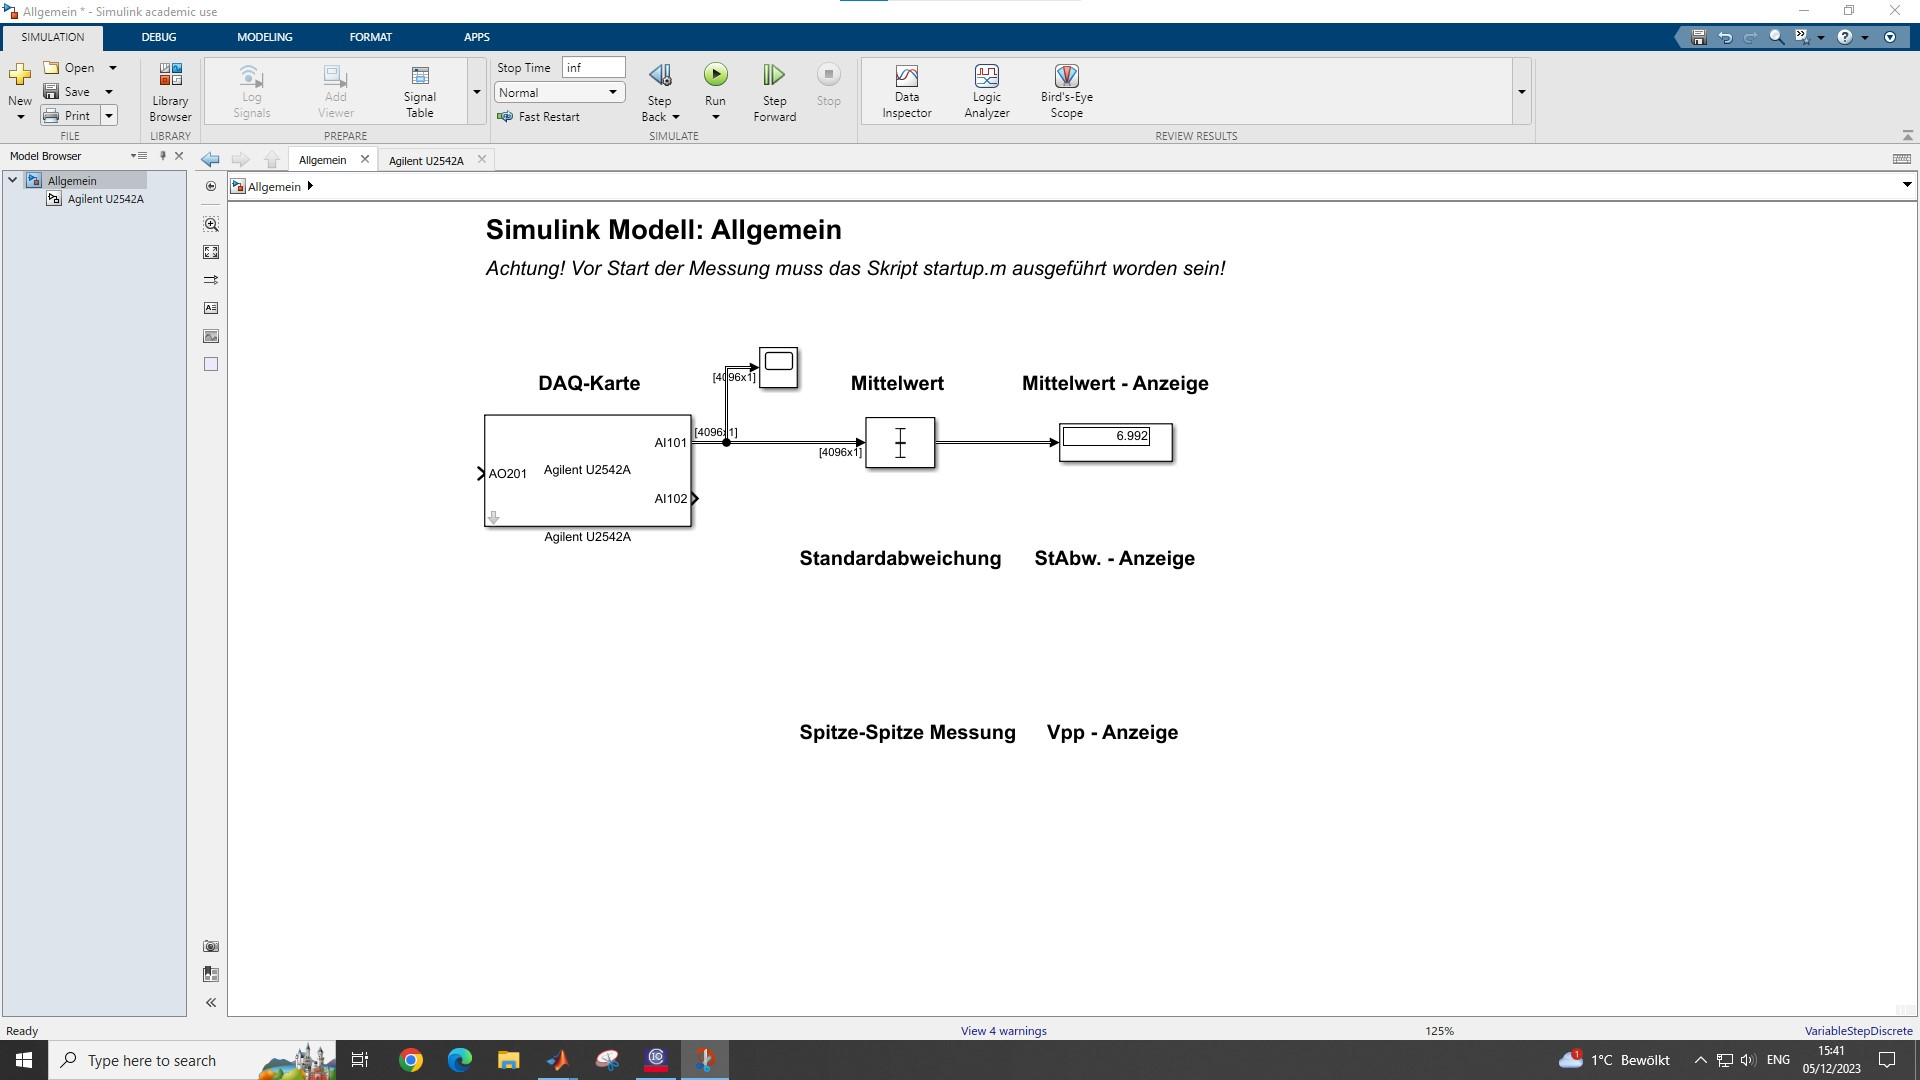
\includegraphics[width=0.8\textwidth]{schematics/schaltung_nur_mean.jpg}
    \caption{Schaltung zur Berechnung von $u_{mean}$}
    \label{fig:umean}
\end{figure}

\subsection{Messergebnisse}
Es konnte direkt zu Beginn festgestellt werden, dass die maximale Ausgangsspannung
des Näherungssensors nicht erreicht werden kann und dass die maximal möglich
Auslenkung der Messschraube $x_{max}=9 \frac{3}{4} \frac{1}{12}''$ beträgt.
Die grobe Messung wurde in $\frac{1}{12}''$-Schritten durchgeführt und lieferte
das Ergebnis aus Tabelle \ref{6-3-2-grobeMessungen}. Daraus ist ersichtlich, dass
 sich das Maximum der Kennlinie bei einer Auslenkung von
$x_{max}\approx \frac{8}{12}''$ befindet, daher wurde die feine Aufnahme
symmetrisch um diesen Punkt herum in $\frac{1}{4}$-Inkrementierungen aufgenommen,
wie in Tabelle \ref{6-3-2-feineMessungen} ersichtlich.
Die gleichen Messungen wurden auch für den zweiten Reflektor RF2 durchgeführt
und sind daher auch in den Tabellen \ref{6-3-2-grobeMessungen} und Tabelle \ref{6-3-2-feineMessungen}
zu finden. An den rechten Enden der Kennlinien aus Abb. \ref{fig:6-3-2-RF1} und
Abb. \ref{fig:6-3-2-RF2} ist deutlich eine steile Erhöhung nach einem kleinen
lokalen Minimum zu erkennen. Das ist vermutlich ein Resultat der Geometrie des
Gehäuses des Näherungssensors. Das Gehäuse ragt weiter aus als die Lichtquelle
des Sensors es tut, daher wird ab einer gewissen Nähe ein geschlossener Raum um
den Sensor gebildet und es wird mehr Licht zum Sensor reflektiert.

\begin{minipage}[t]{0.5\textwidth}
    \centering
    \captionof{table}{grobe Aufnahme der Kennlinie}
    \label{6-3-2-grobeMessungen}
    \begin{tabular}{|c|c|c|}
        \hline
        $x \unit{[\frac{1}{12}'']}$&  $u_{mean,RF1}\unit{[V]}$ &$u_{mean,RF2}\unit{[V]}$ \\
        \hline
        0,00 & 0,06213 &  0.2089\\
        1,00  & 0,06885 &  0.2717\\
        2,00  & 0,08384 &  0.3744\\
        3,00  & 0,1094  &   0.5481\\
        4,00  & 0,1558  &   0.8675\\
        5,00  & 0,2479  &   1.5\\   
        6,00  & 0,4343  &   2.838\\ 
        7,00  & 0,7825  &   5.581\\ 
        8,00  & 0,9863  &   7.972\\ 
        9,00  & 0,3565  &   3.281\\ 
        \hline
    \end{tabular}
\end{minipage}
\begin{minipage}[t]{0.5\textwidth}
    \centering
    \captionof{table}{feine Aufnahme der Kennlinie}
    \label{6-3-2-feineMessungen}
    \begin{tabular}{|c|c|c|}
        \hline
        $x \unit{[\frac{1}{12}'']}$&  $u_{mean,RF1}\unit{[V]}$ &$u_{mean,RF2}\unit{[V]}$ \\
        \hline
        5,00   & 0.235     &  1.491\\    
        5,25&     0.2706&      1.731\\
        5,5 & 0.313     &  2.025\\    
        5,75&     0.3644&      2.383\\
        6,00   & 0.4241    &  2.818\\    
        6,25&     0.4958&      3.343\\
        6,5 & 0.579     &  3.969\\    
        6,75&     0.6733&      4.706\\
        7,00   & 0.7759    &  5.542\\    
        7,25&     0.8783&      6.43\\ 
        7,5 & 0.9635    &  7.271\\    
        7,75&     1.007 &      7.868\\
        8,00   & 0.9916    &  7.995\\    
        8,25&     0.8739&      7.371\\
        8,5 & 0.6738    &  5.933\\    
        8,75&     0.4646&      4.224\\
        9,00   & 0.351     &  3.278\\    
        9,25&     0.3851&      3.787\\
        9,5 & 0.3736    &  4.766\\    
        \hline
    \end{tabular}
\end{minipage}

\begin{figure}[h]
    \centering
    \begin{minipage}{0.45\textwidth}
        \centering
        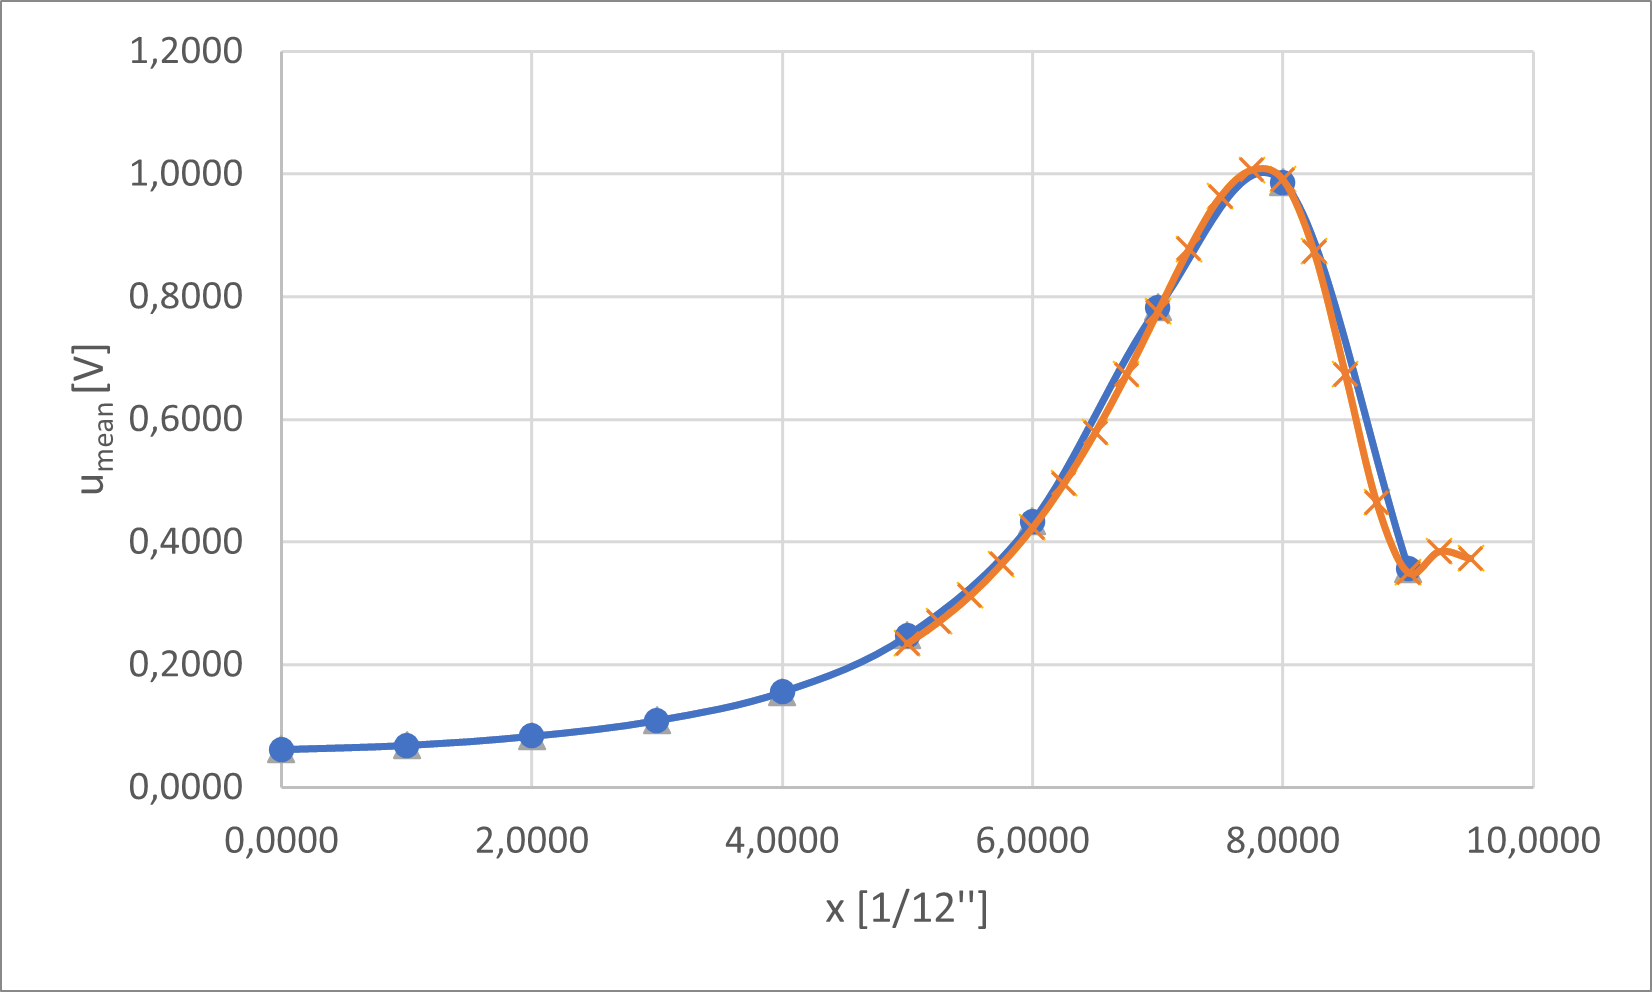
\includegraphics[width=1.0\textwidth]{images/6-3-2-Reflektor1.png}
        \caption{Kennlinie vom Reflektor RF1}
        \label{fig:6-3-2-RF1}
    \end{minipage}
    \centering
    \begin{minipage}{0.45\textwidth}
        \centering
        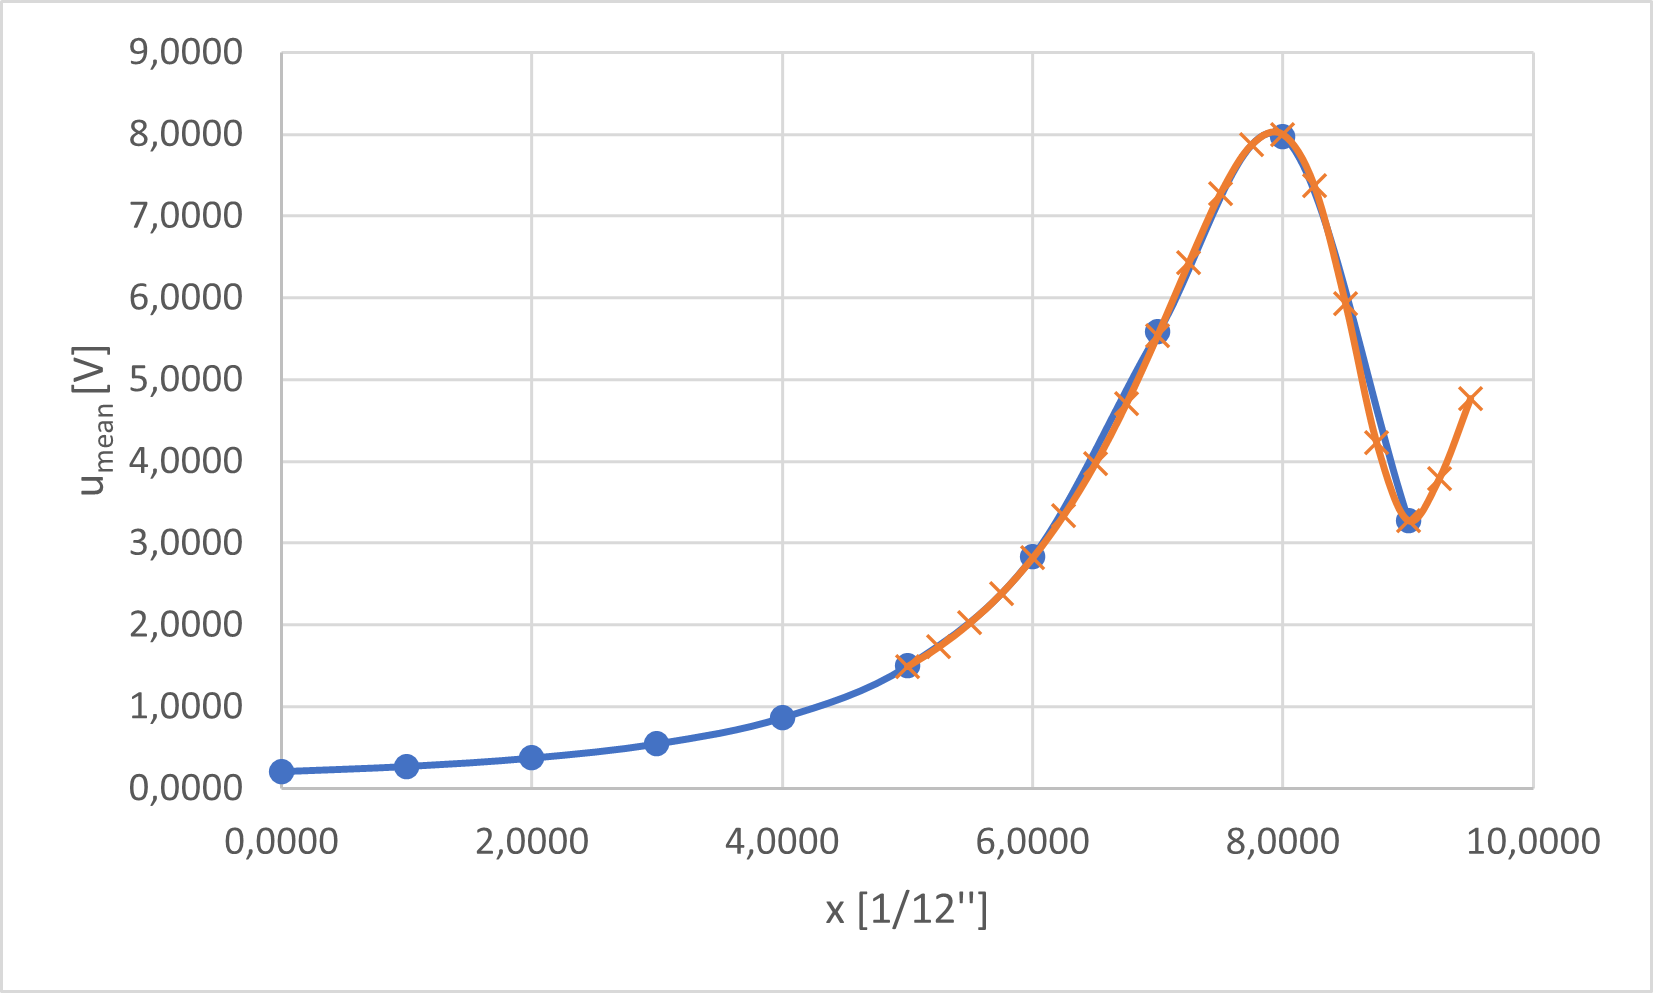
\includegraphics[width=1.0\textwidth]{images/6-3-2-Reflektor2.png}
        \caption{Kennlinie vom Reflektor RF2}
        \label{fig:6-3-2-RF2}
    \end{minipage}
\end{figure}

\section{Rauschen und Auflösung}
Zur Rauschmessung wird die Schaltung beibehalten wie sie ist, es wird lediglich
der stärker reflektierende Reflektor RF2 verbaut und der Abstand der größten
Signalamplitude eingestellt. Zusätzlich wird das Blockschaltbild um die
Berechnung der Standardabweichung sowie der Spitze-Spitze-Spannung wie in
\reg{fig:schematics-6-3-3-jpg} erweitert.\newline
Die Umgebungsbedingungen während der Messung waren:
\begin{izemize}
    \item vollständige Deckenbeleuchtung
    \item kein Schattenwurf auf das Messobjekt
    \item kein Sonnenlicht, helle Wolkendecke um 15Uhr in Wien 
\end{izemize}

\begin{figure}[h]
    \centering
    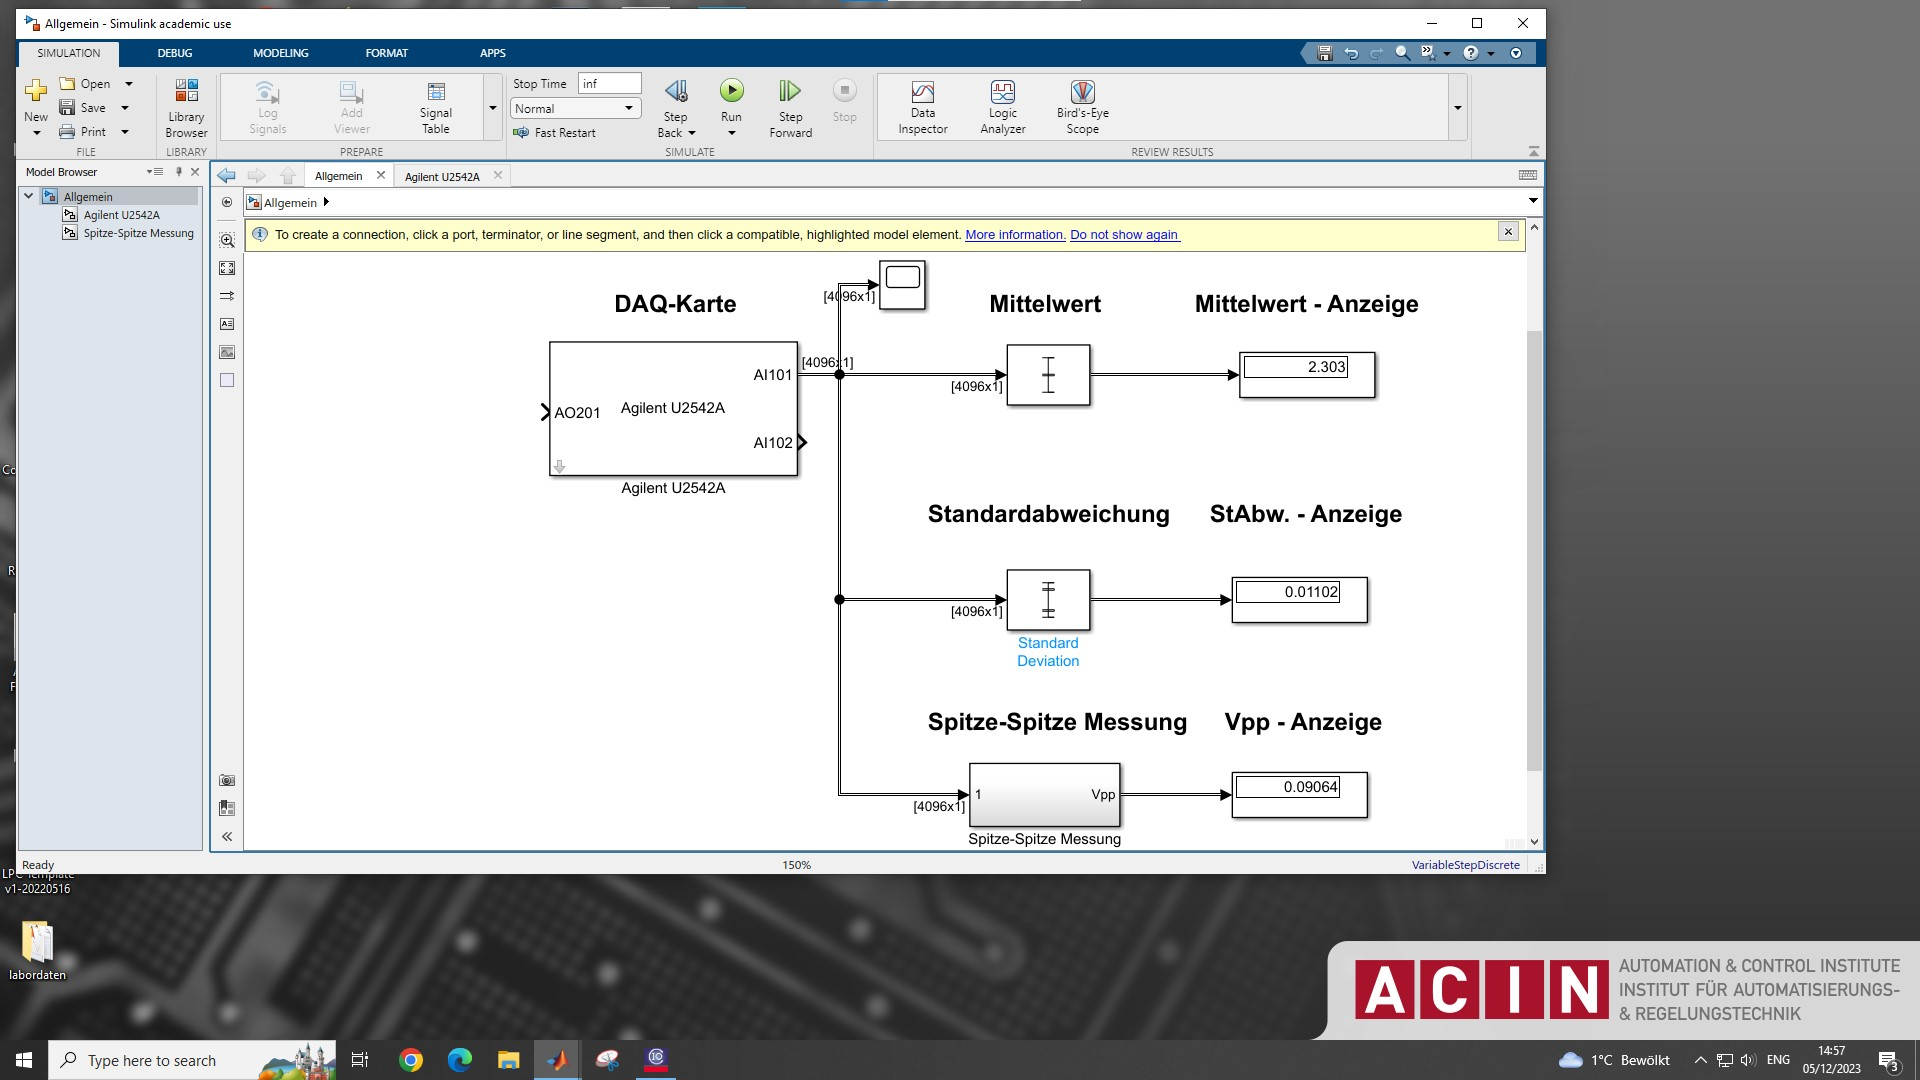
\includegraphics[width=0.8\textwidth]{schematics/6.3.3).jpg}
    \caption{Erweiterung um Standardabweichung und Spitze-Spitze-Wert}
    \label{fig:schematics-6-3-3-jpg}
\end{figure}

\subsection{Messergebnisse}
Wie aus den Ergebnissen aus der Tabelle \ref{tab:6-3-3} zu sehen ist, scheint
die angelegt Spannung kaum dem Rauschen beizutragen. Die mittlere Spannungs ist
jedoch wie zu erwarten gefallen. Die größten Quellen für das Rauschen werden
vermutlich Lichtquellen ausmachen. Zu den Rauschquellen gehört die Strahlung die
von Außen wirkt, die Deckenbeleuchtung und das Grundrauschen der Schaltung durch
die Spannungsversorgung. Denkbar wären auch Luftverschmutzung wie Staub und
Feuchtigkeitsschwankungen in der Luft, die mit der Lichtquelle der Schaltung
interferieren.

\begin{table}[h]
    \centering
    \caption{Messergebnisse der Standardabweichung, Spitze-Spitze-Werte und dem Mittelwert}
    \label{tab:6-3-3}
    \begin{tabular}{|c|c|c|c|}
        \hline
        \multicolumn{4}{|c|}{Input $1,5\unit{V_{DC}}$}\\
        \hline
        $t\unit{[s]}$ & $u_{mean}\unit{[V]}$ & $\sigma(u)\unit{[V]}$ &  $u_{pp}\unit{V}$ \\
        \hline
        10&8,264&0,01234&0,1077\\
        60 & 8,258 & 0,01251 & 0,1068\\
        120 & 8,258 & 0,01235 & 0,1071\\
        \hline
        \hline
        \multicolumn{4}{|c|}{Input $0,5\unit{V_{DC}}$}\\
        \hline
        $t\unit{[s]}$ & $u_{mean}\unit{[V]}$ & $\sigma(u)\unit{[V]}$ &  $u_{pp}\unit{V}$ \\
        \hline
        10  & 2,248 & 0,01144 & 0,09277\\
        60 & 2,257 & 0,01131 & 0,09094\\
        120 & 2,262 & 0,01113 & 0,08972\\
        \hline
    \end{tabular}
\end{table}

\section{Sepktrum der Fremdlichtintensität}
Nun sollen Fremdlichtquellen untersucht werden, weshalb die Versorgung der
Lichtquelle des Näherungssensors über den Funktionsgenerator ausgeschaltet wurde
und das Simulink-Blockschaltbild um einen Spectrum-Analyzer erweitert wurde
(siehe Abb. \ref{fig:6-3-4-Simulink}). Die Einstellungen des Spectrum-Analyzers
wurden dem Skriptum entnommen (Type: RMS, Span: $2000 \unit{Hz}$, Units:  $dBV$, Trace-options: off).
Als konstante Lichtquelle wurde die Glühfadenlampe LA1 aus einer Entfernung von
$25\unit{cm}$ eingesetzt ohne einen Schatten auf den Sensor zu projizieren.
Es wurden sowohl die Spektren als auch das Rauschen in unterschiedlichen Situationen
gemessen.

\begin{figure}[h]
    \centering
    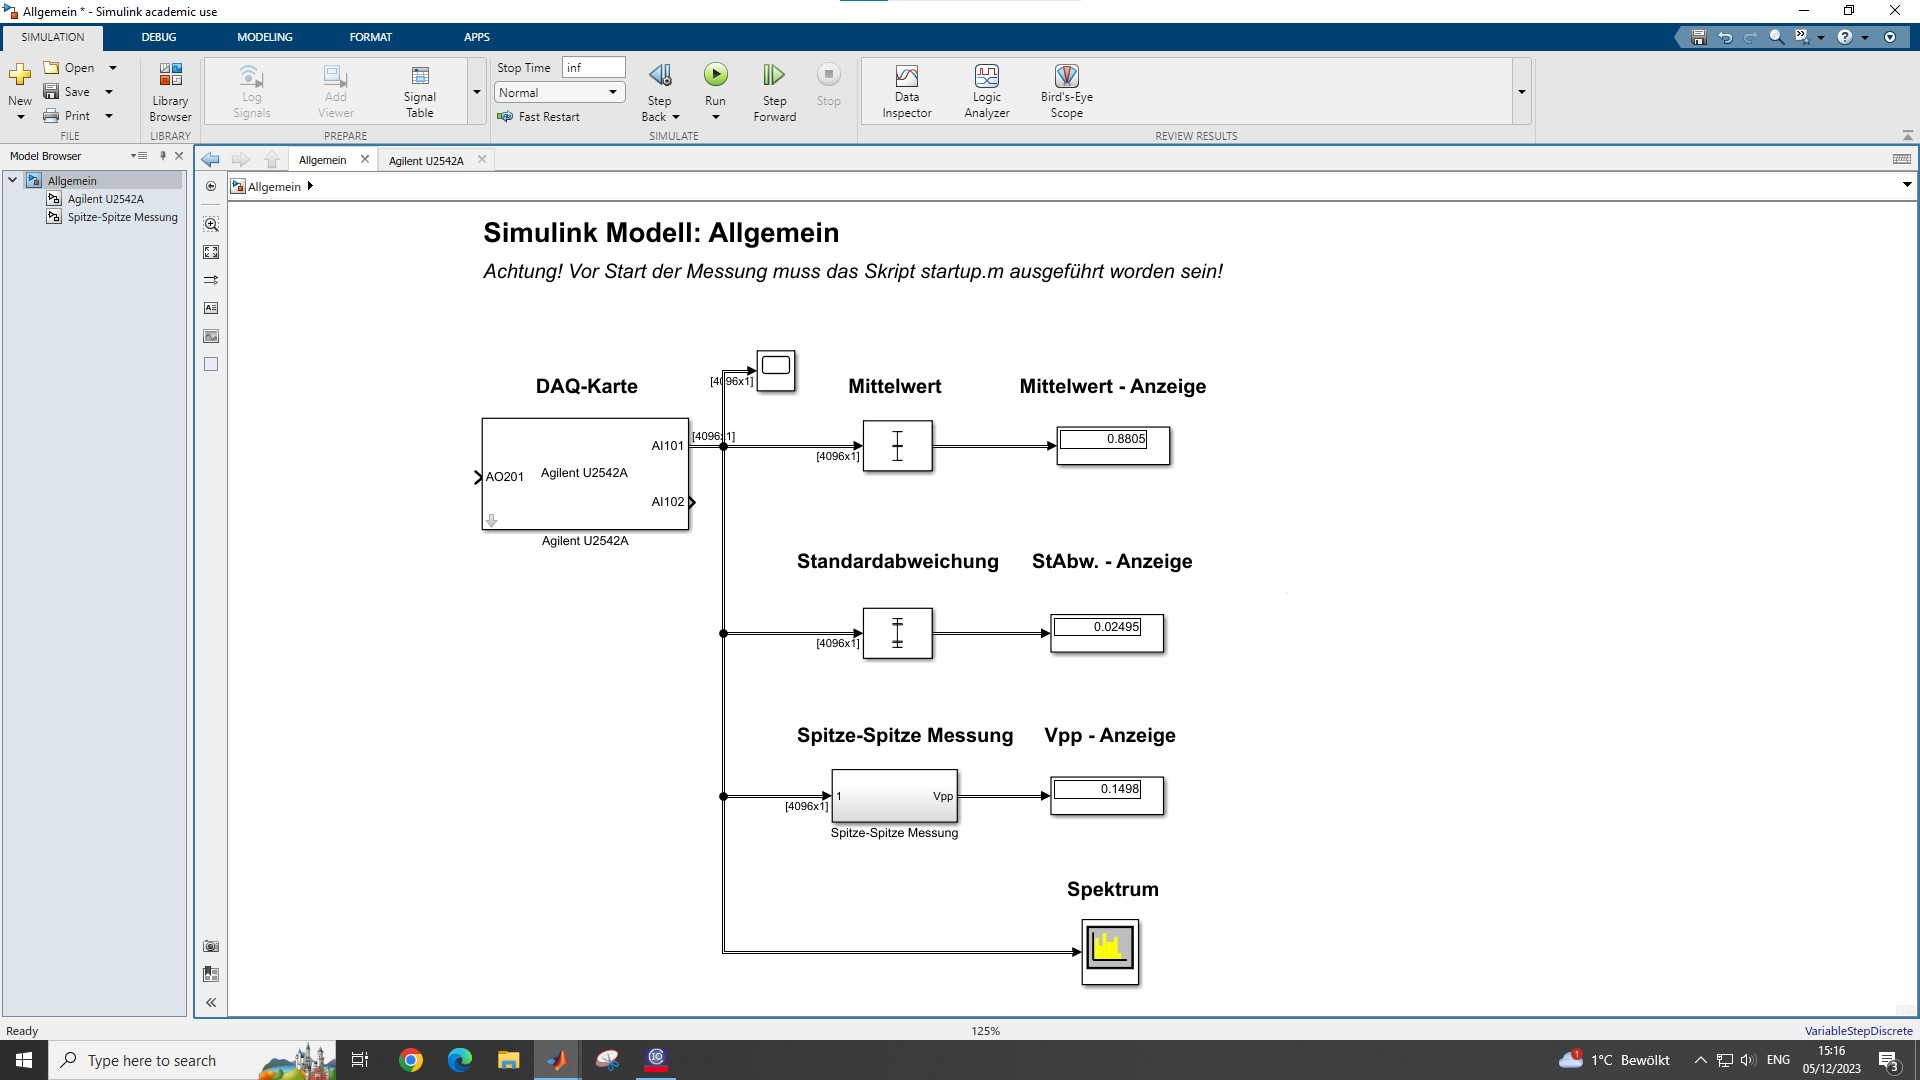
\includegraphics[width=0.8\textwidth]{schematics/6.3.4)spektrum_schaltung.jpg}
    \caption{Erweitertes Simulink Blockschaltbild}
    \label{fig:6-3-4-Simulink}
\end{figure}


\subsection{Messergebnisse}
Wie zu erwarten ist die mittlere Spannung extrem stark von der Fremdlichtintensität
abhängig. Wenn die Lampe ausgeschaltet wird, fällt $u_{mean}$ um eine Größenordnung
und wenn der Sensor abgedeckt wird, fällt es sogar um eine weitere Größenordnung.
Bei der Standardabweichung ist so ein Verhalten nicht beobachtbar, die Spitze-Spitze-Spannung
hat jedoch eine leichte Abhängigkeit von der Fremdlichtintensität. Wenn man
die Frequenz-Analyse betrachtet, kann man aus dem Vergleich von Abb. \ref{fig:6-3-4-mitLA1}
und Abb. \ref{fig:6-3-4-ohneLA1} erkennen, dass die diffuse Strahlung den Großteil
der Fremdintensität ausmacht. Weiters lässt sich das Frequenzspektrum der Lampe
sehr leicht identifizieren, da der Peak fast genau $100\unit{Hz}$ auftritt.
Das entspricht der doppelten Netzfrequenz und somit genau der Frequenz der Leistung.

\begin{table}[h]
    \centering
    \caption{Messergebnisse der Standardabweichung, Spitze-Spitze-Werte und dem Mittelwert}
    \label{tab:6-3-4}
    \begin{tabular}{|c|c|c|c|}
        \hline
        \multicolumn{4}{|c|}{Lampe bei $t=0\unit{s}$ eingeschaltet}\\
        \hline
        $t\unit{[s]}$ & $u_{mean}\unit{[V]}$ & $\sigma(u)\unit{[V]}$ &  $u_{pp}\unit{[V]}$ \\
        \hline
        5&0,2684&0,01346&0,1013\\
        50 & 0,2699& 0,013 & 0,1028\\
        80 & 0,2777 & 0,01283 & 0,1028\\
        120 & 0,2741 & 0,01314 & 0,1028\\
        \hline
        \hline
        \multicolumn{4}{|c|}{Lampe bei $t=0\unit{s}$ ausgeschaltet}\\
        \hline
        $t\unit{[s]}$ & $u_{mean}\unit{[V]}$ & $\sigma(u)\unit{[V]}$ &  $u_{pp}\unit{[V]}$ \\
        \hline
        90 & 0,02478 & 0,0113 & 0,08545\\
        120 & 0,0248 & 0,0112 & 0,08484\\
        \hline
        \hline
        \multicolumn{4}{|c|}{abgedeckte Schaltung}\\
        \hline
        $t\unit{[s]}$ & $u_{mean}\unit{[V]}$ & $\sigma(u)\unit{[V]}$ &  $u_{pp}\unit{[V]}$ \\
        \hline
        10 & 0,004232 & 0,01132 & 0,08545\\
        45 & 0,0003277 & 0,01169 & 0,08545\\
        90 & 0,0003546 & 0,01126 & 0,08514\\
        \hline
    \end{tabular}
\end{table}
\begin{figure}[h]
    \centering
    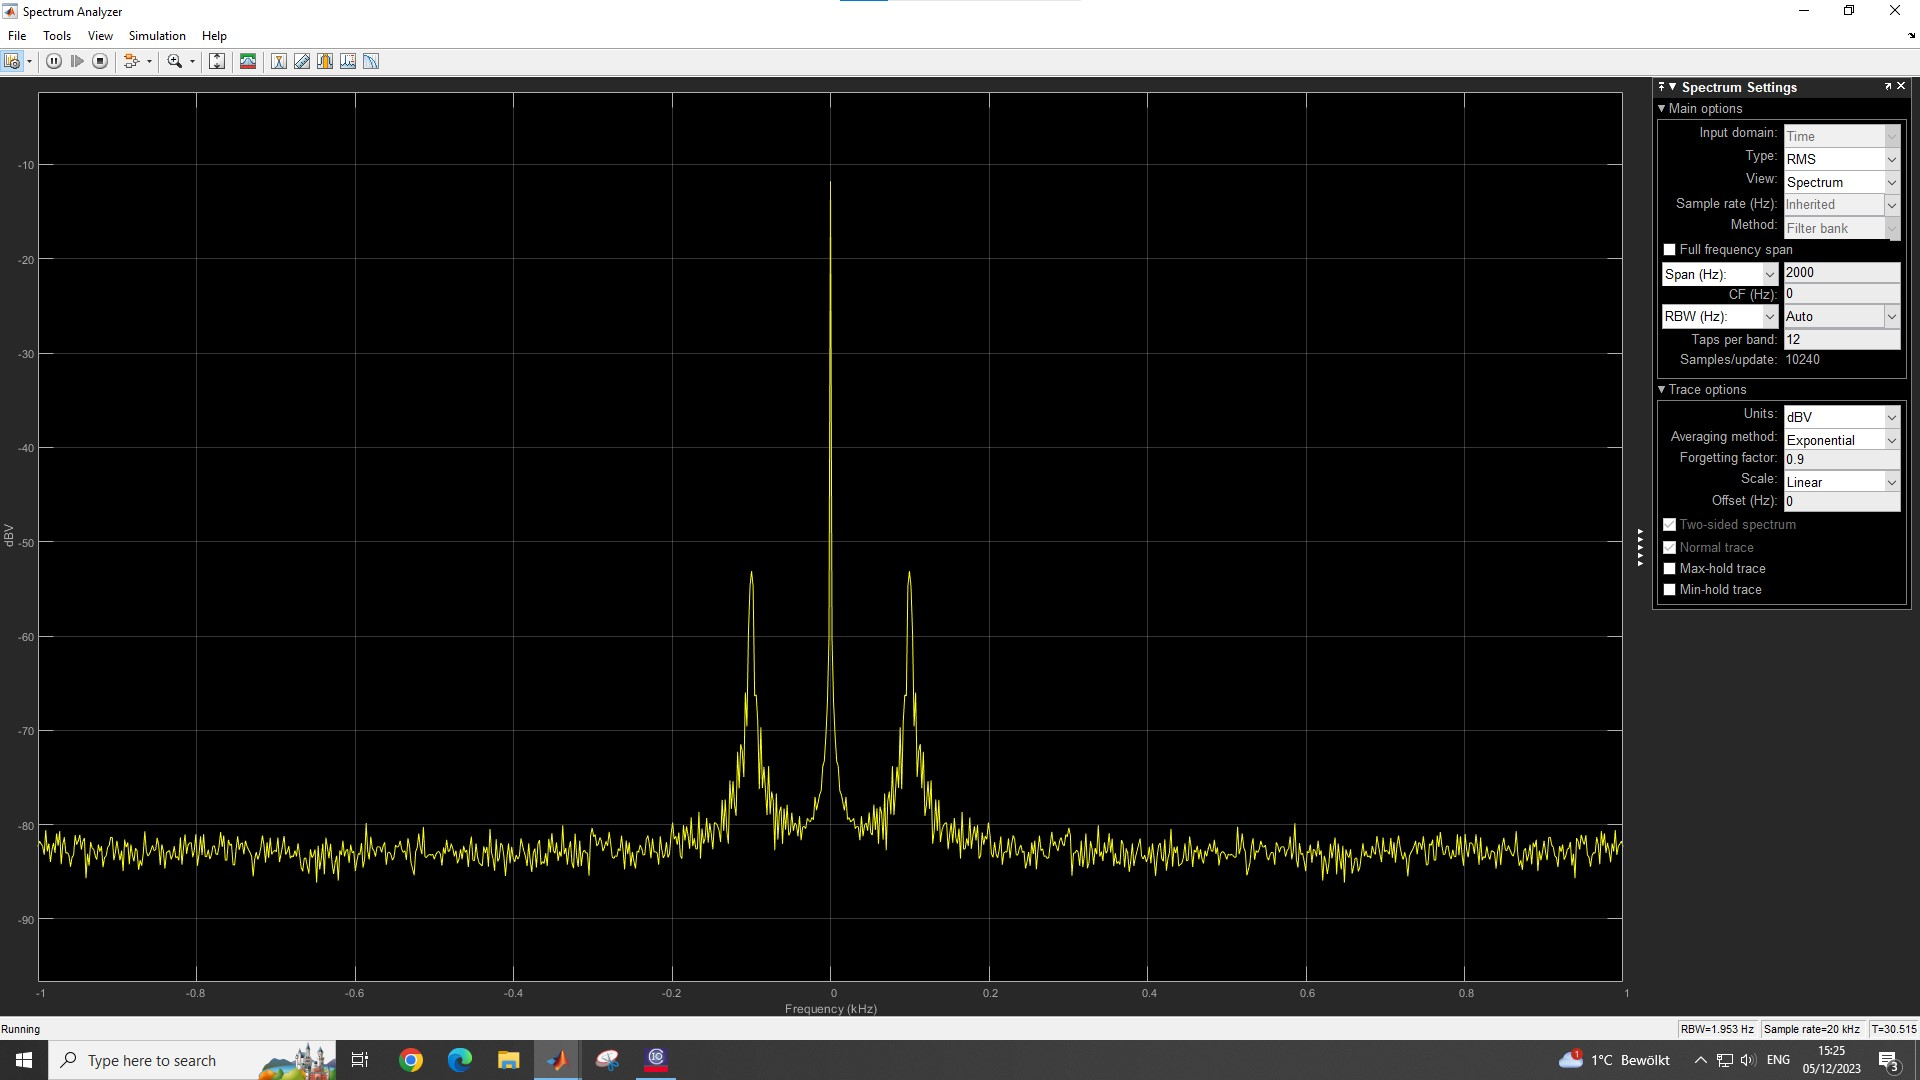
\includegraphics[width=0.8\textwidth]{images/6.3.4)mit_lampe.jpg}
    \caption{Frequenzspektrum mit eingeschalteter Lampe}
    \label{fig:6-3-4-mitLA1}
\end{figure}
\begin{figure}[h]
    \centering
    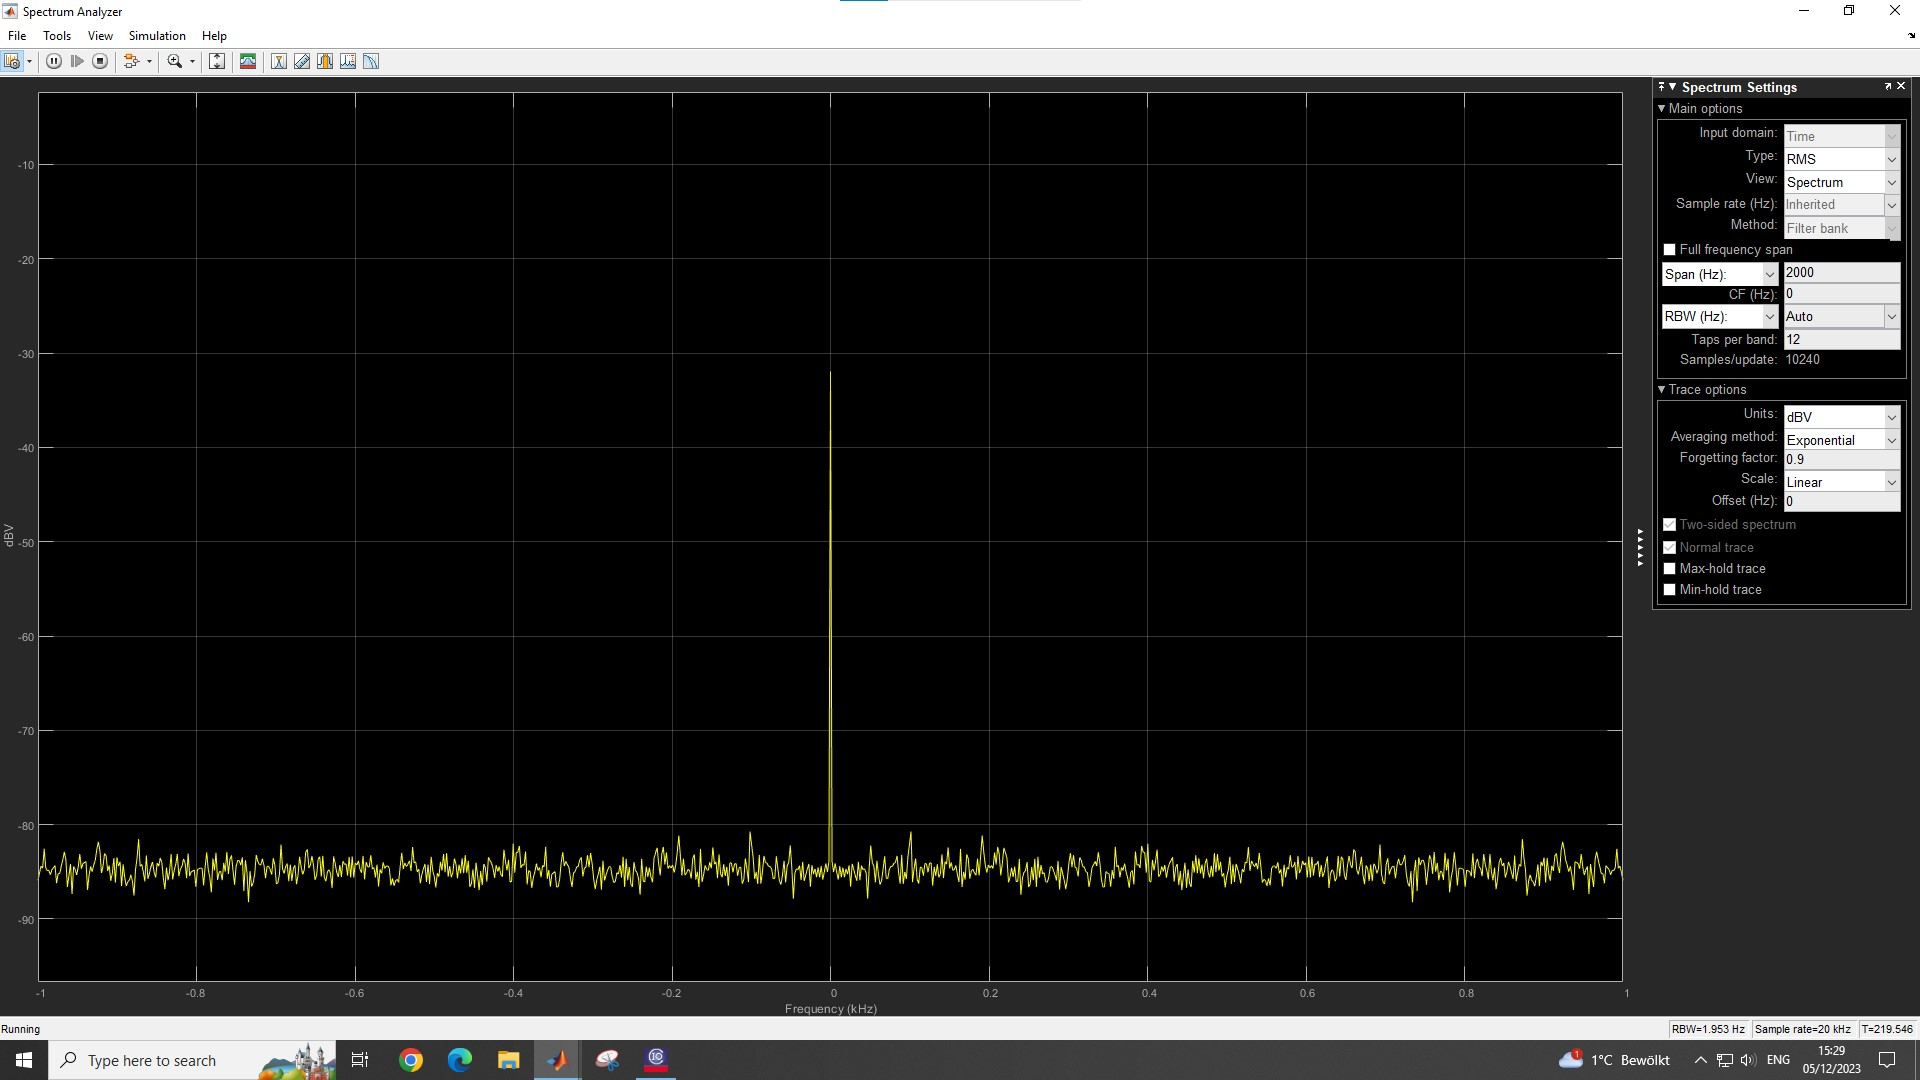
\includegraphics[width=0.8\textwidth]{images/6.3.4)ohne_lampe.jpg}
    \caption{Frequenzspektrum mit eingeschalteter Lampe}
    \label{fig:6-3-4-ohneLA1}
\end{figure}

\section{Phasenselektiver Synchrongleichrichter}
Der Ausgang des Funktionsgenerators FG1 wurde auf ein Sinussignal ($U_{pp}=0,4\unit{V}$,
$U_{offset}=1,3\unit{V}$) gestellt und zusätzlich am Eingang AI102 angeschlossen.
Weiters wurde der Ausgang des Sensors, welcher an AI101 angeschlossen ist, mit dem
Oszilloskop überwacht. Es wurde weiterhin der Reflektor RF2 verwendet.\newline
Das Simulink-Blockschaltbild wurde wie im Skriptum beschrieben erweitert und mit
einem Butterworth-Tiefpassfilter zehnter Ordnung ($f_{g}=3\unit{Hz}$ ) ausgestattet,
siehe Abb. \ref{fig:6-3-5-schaltung}. Die Werte für die Phasenverschiebung (in der Schaltung
Abb. \ref{fig:6-3-5-schaltung} mit $d$ eingetragen) wurden in der Labor-Hausübung
berechnet und hier für je $45^\circ$ und  $90^\circ$ übernommen. \newline
Nachdem das Blockschaltbild vervollständigt wurde, wurde die Lampe auf $15\unit{cm}$
Entfernung positioniert und die Ausgangsamplitude auf $1 V_{pp}$ gestellt.
Letztendlich wurden alle Messwerte aufgenommen.

\begin{figure}[h]
    \centering
    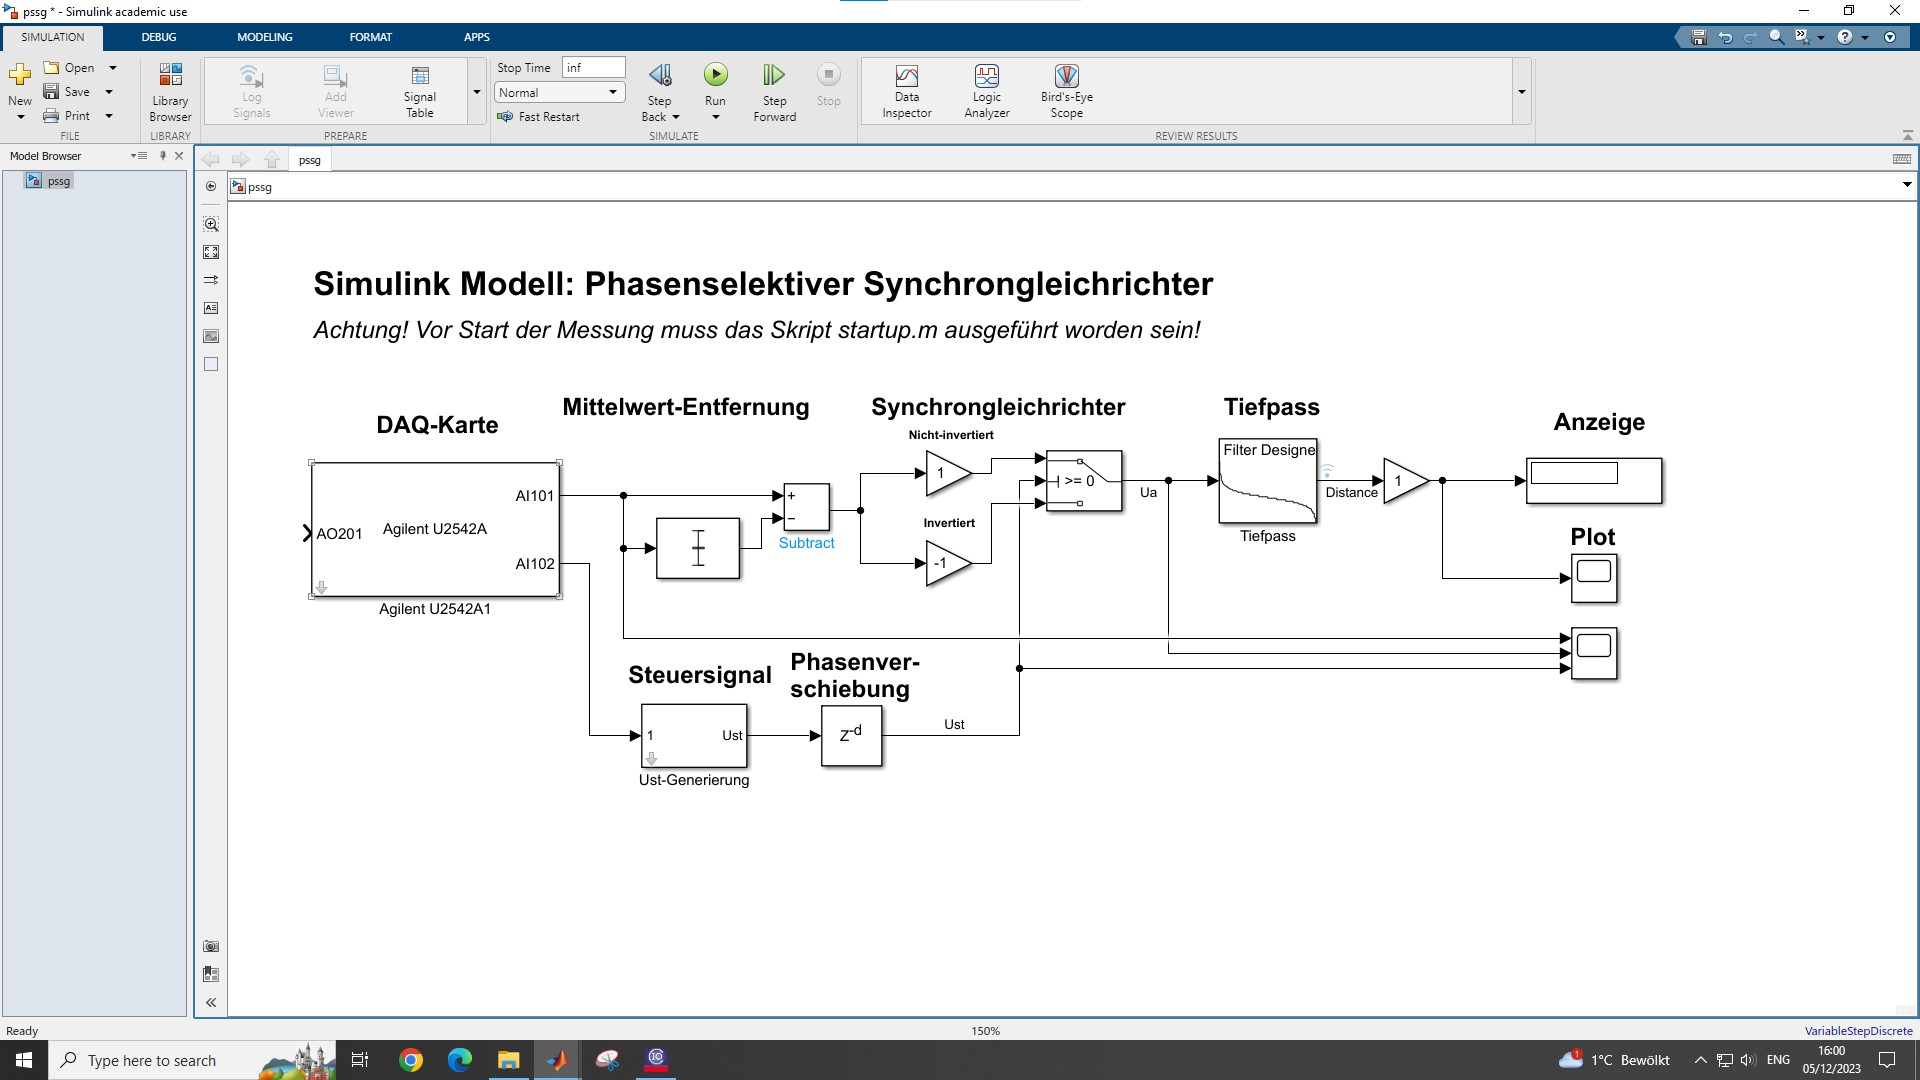
\includegraphics[width=0.8\textwidth]{schematics/6.3.5)schaltung.jpg}
    \caption{Schaltung des phasenunabhängigen Synchrondemodulators}
    \label{fig:6-3-5-schaltung}
\end{figure}

\subsection{Messergebnisse}
Wir erwarten dann Oberwellen, wenn Frequenzdifferenz zwischen Störsignalfrequenz
und Ausgangssignal kleiner als unsere Grenzfrequenz $f_{g}=3\unit{Hz}$ ist.

\begin{table}[h]
    \centering
    \caption{Korrespondenztabelle zwischen Störsignal und Frequenz}
    \label{tab:6-3-5-störfrequenz}
    \begin{tabular}{|c||c|c|c|}
        \hline
        Frequenz (Hz) & Störung erwartet? & Störung gemessen? & Begründung \\
        \hline
        20\pm 0,1 & Nein & Nein & Frequenzdifferenz zu hoch\\
        33,33 \pm 0,1 & Nein & Nein & Frequenzdifferenz zu hoch\\
        50 \pm 0,1 & Nein & Nein & Frequenzdifferenz zu hoch\\
        75 \pm 0,1 & Nein & Nein & Frequenzdifferenz zu hoch\\
        100 \pm 0,1 & Ja & Ja & Frequenzdifferenz: $\Delta f=f - f_{Netz} = 0,1\unit{Hz}$\\
        125 \pm 0,1 & Nein & Nein & Frequenzdifferenz zu hoch\\
        150 \pm 0,1 & Nein & Nein & Frequenzdifferenz zu hoch\\
        175 \pm 0,1 & Nein & Nein & Frequenzdifferenz zu hoch\\
        200 \pm 0,1 & Nein & Nein & Frequenzdifferenz zu hoch\\
        \hline
    \end{tabular}
\end{table}

\begin{figure}[h]
    \centering
    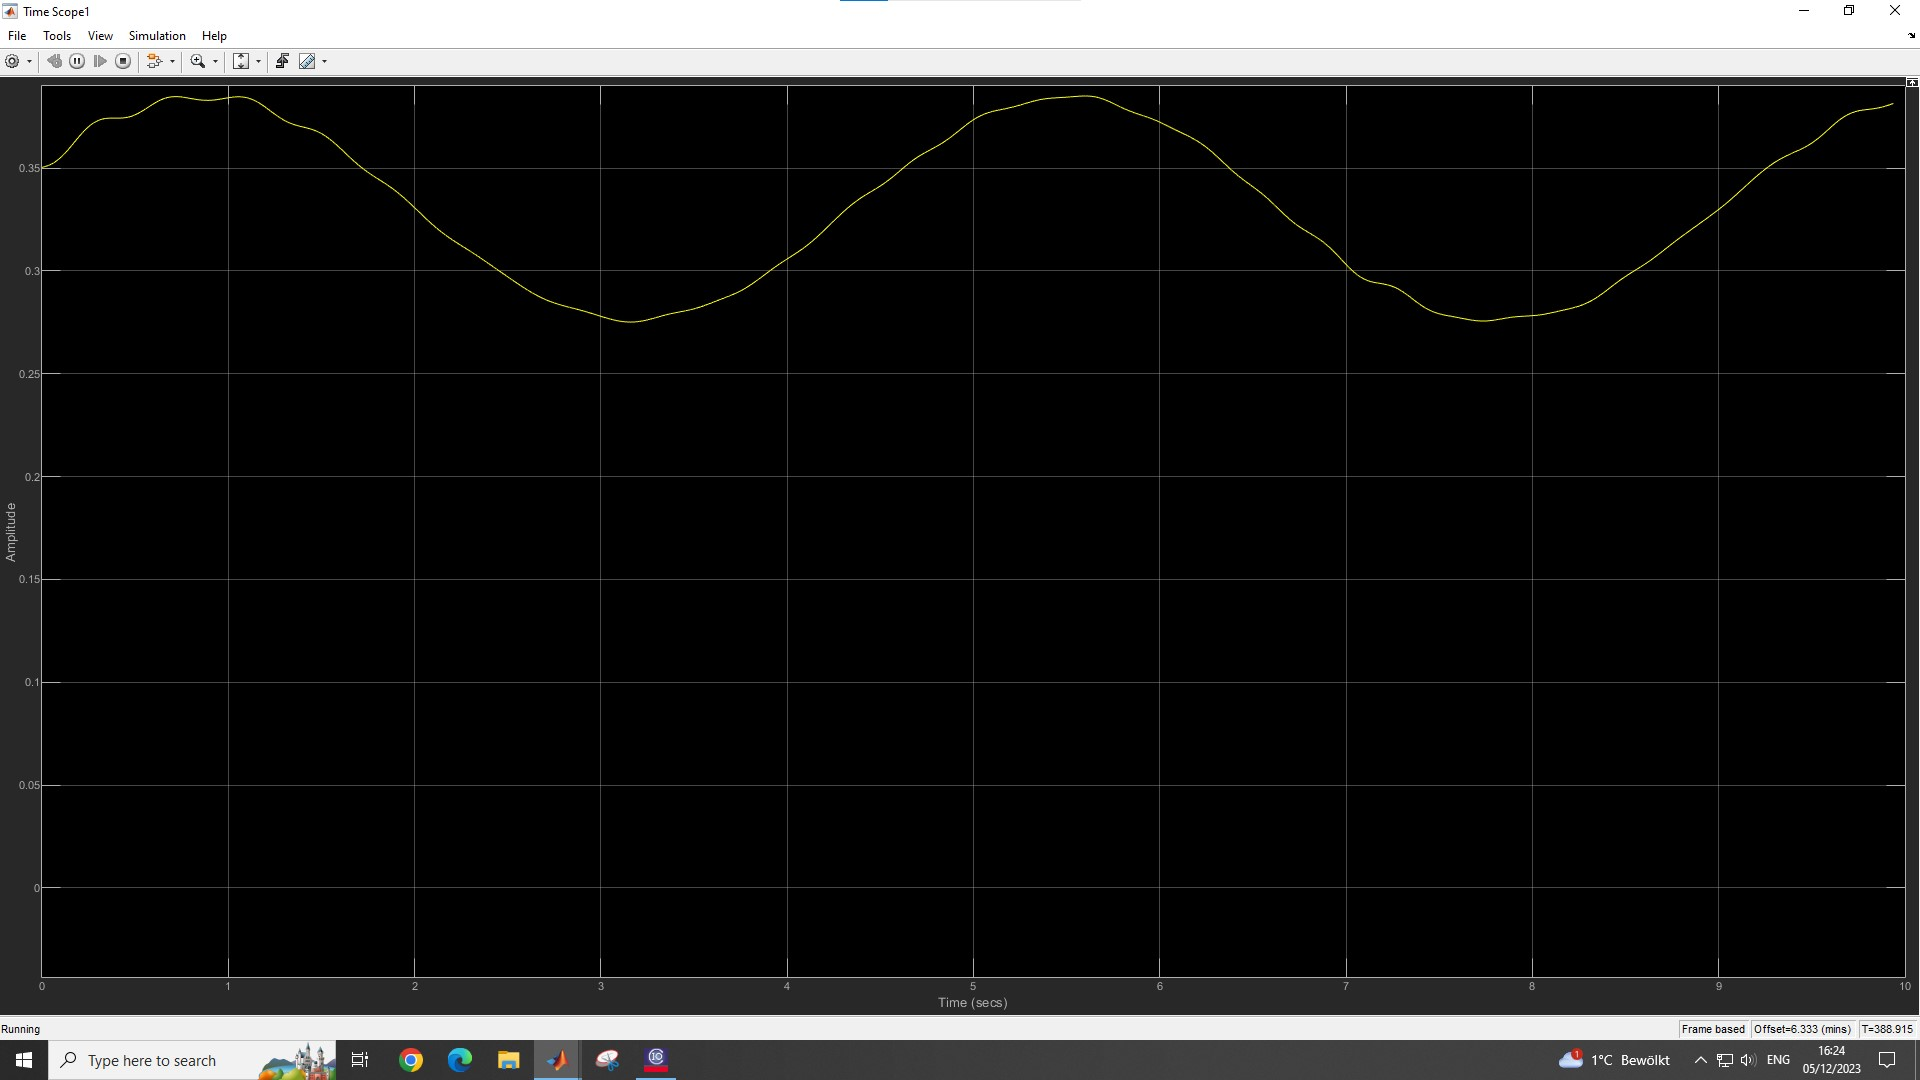
\includegraphics[width=0.8\textwidth]{images/6.3.5)gleichrichter_0grad+lampe_ausgang100,1hz.jpg}
    \caption{Überlagerte Schwingung bei $f=100,1\unit{Hz}$}
    \label{fig:6-3-5-0grad-mitLA1-1001hz}
\end{figure}

\begin{figure}[h]
    \centering
    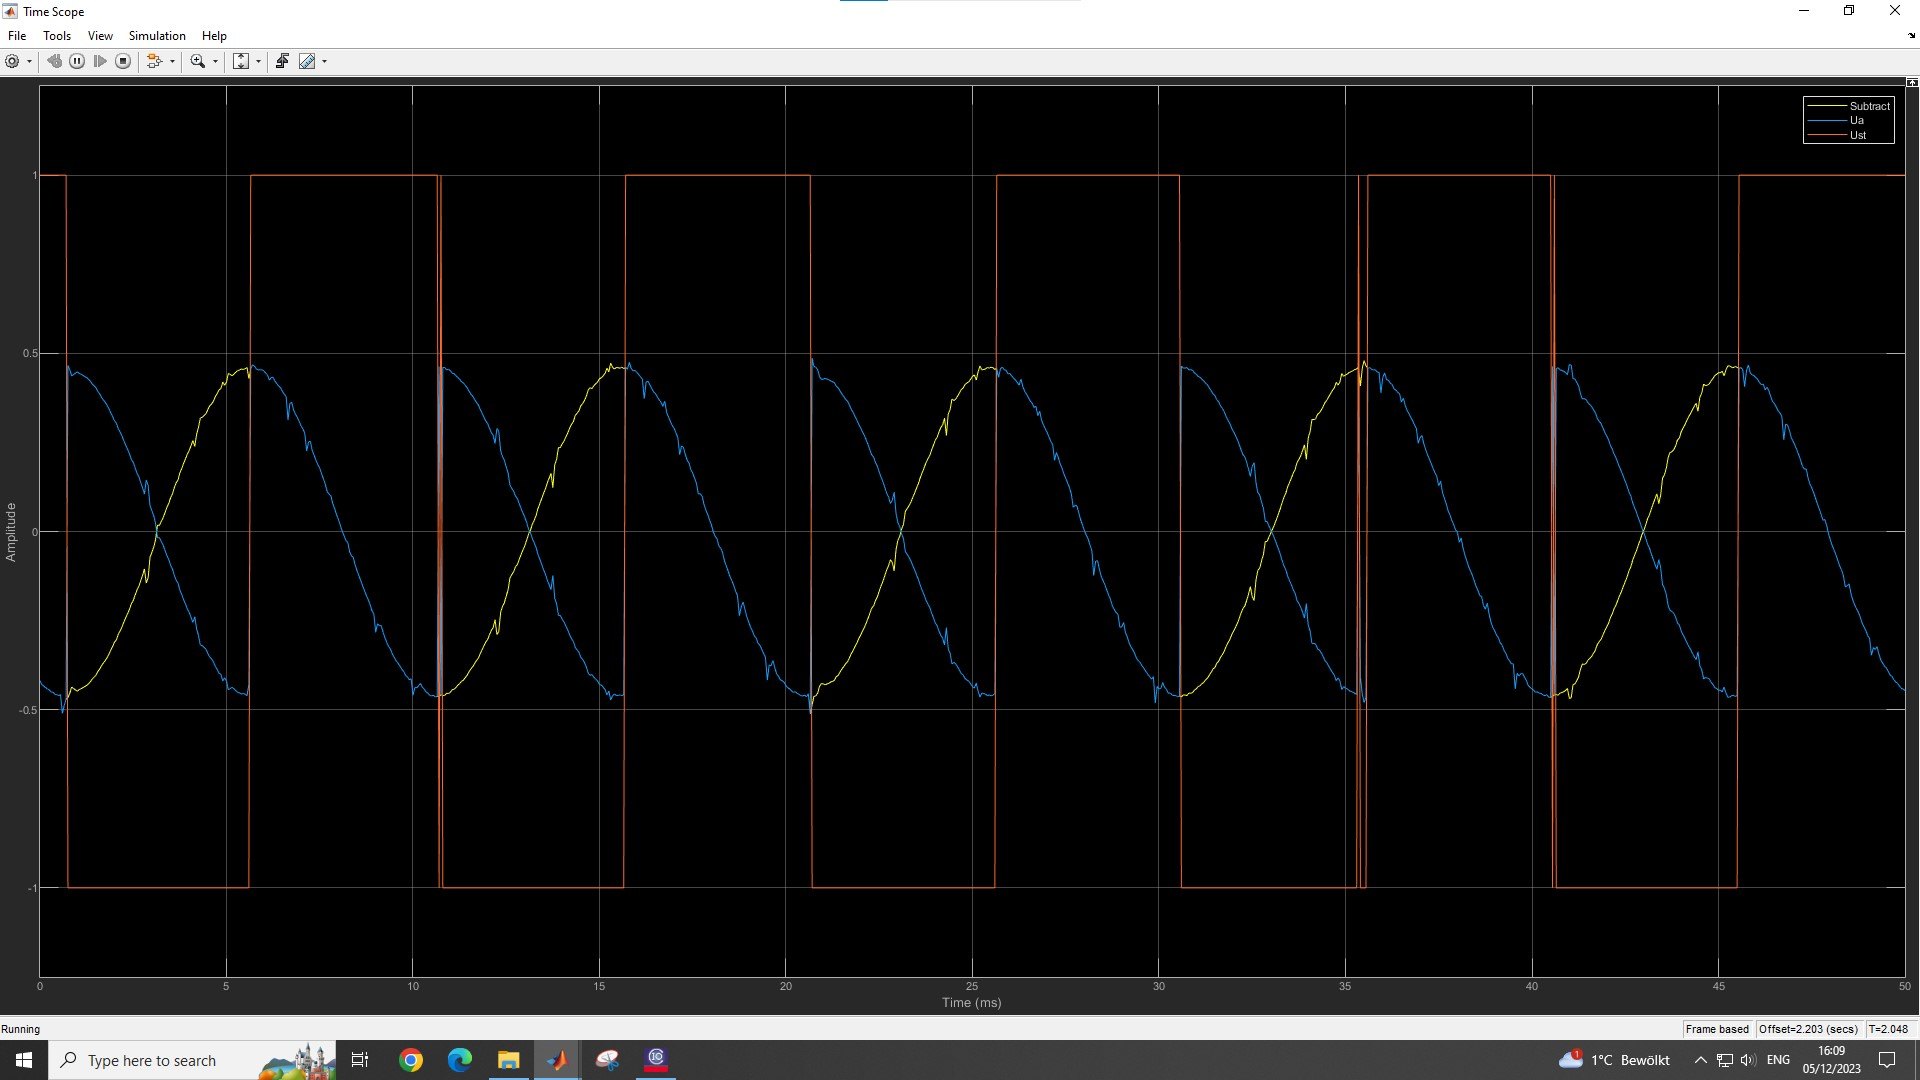
\includegraphics[width=0.8\textwidth]{images/6.3.5)gleichrichter_45gradv2.jpg}
    \caption{Phasenselektiver Synchrongleichrichter bei $45^\circ$ Phasenversatz}
    \label{fig:images-6-3-5-gleichrichter_45gradv2-jpg}
\end{figure}

\begin{figure}[h]
    \centering
    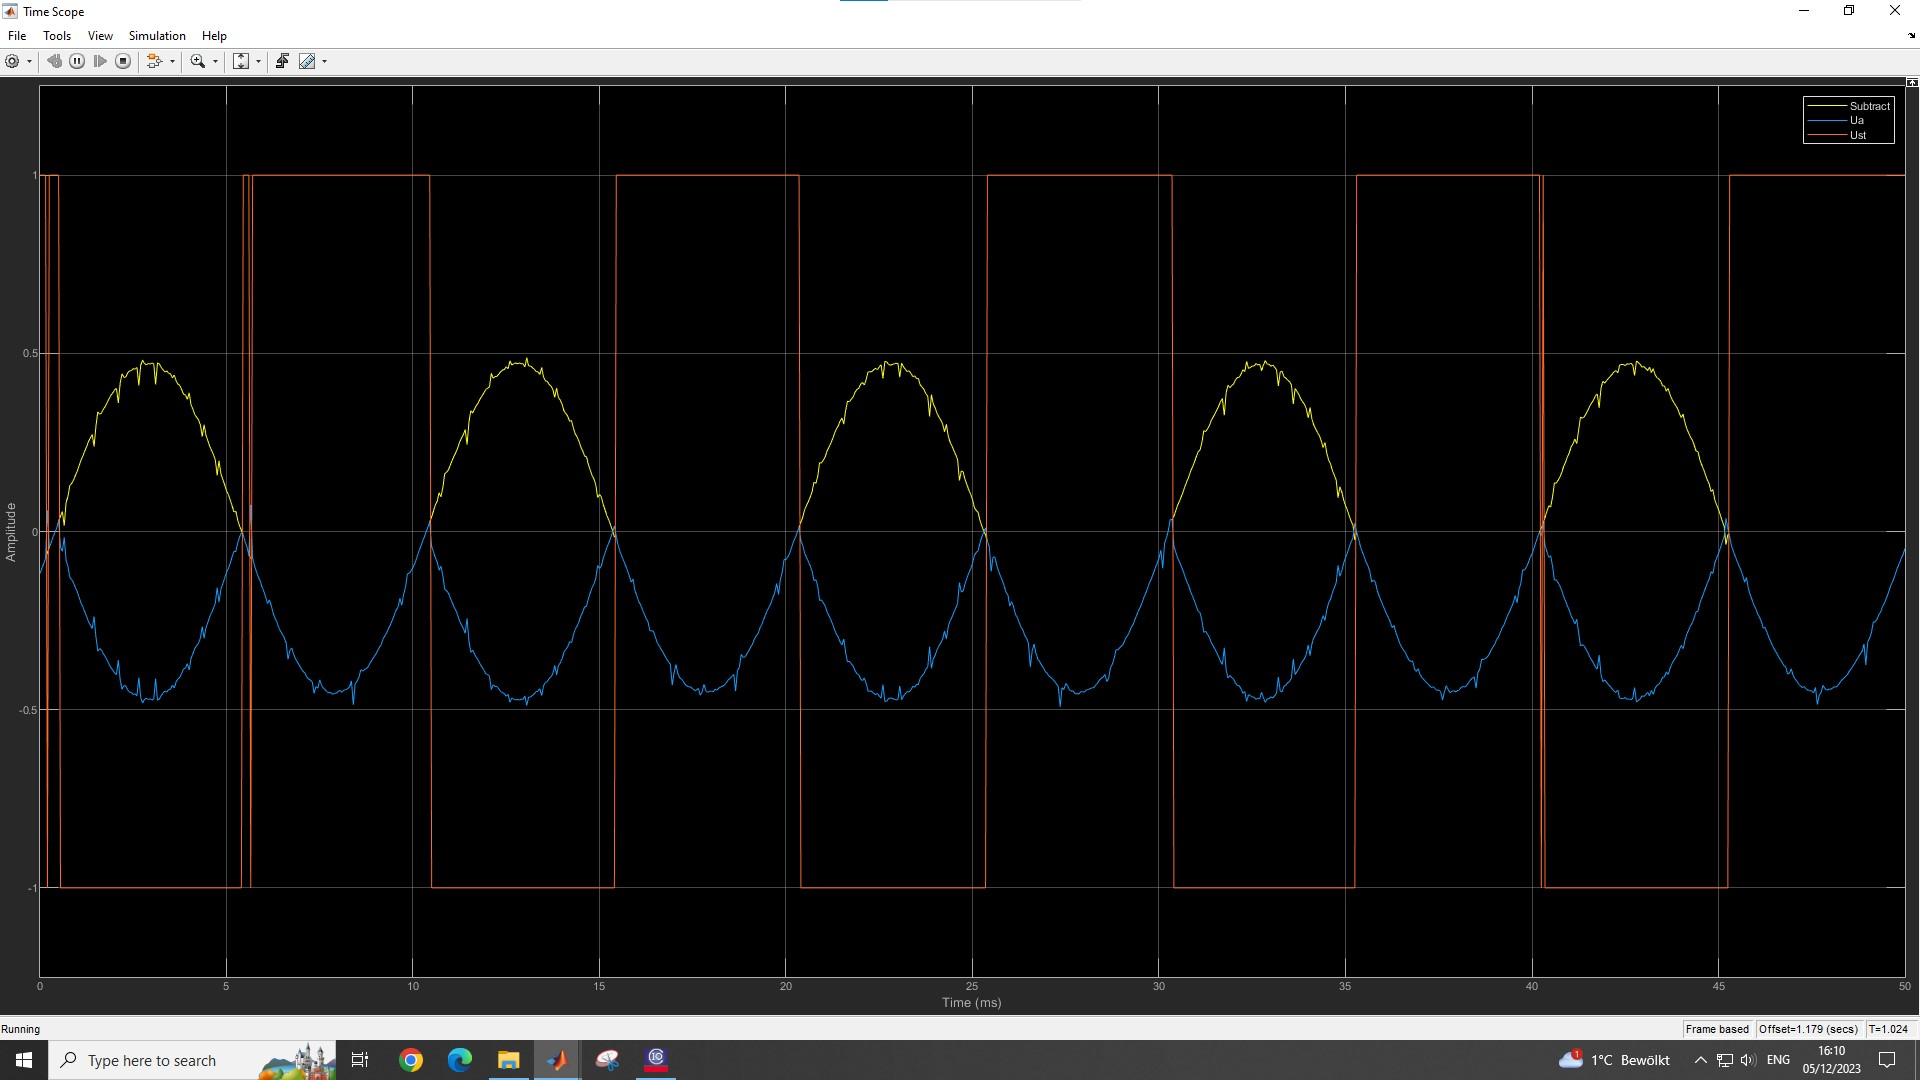
\includegraphics[width=0.8\textwidth]{images/6.3.5)gleichrichter_90gradv2.jpg}
    \caption{Phasenselektiver Synchrongleichrichter bei $90^\circ$ Phasenversatz}
    \label{fig:images-6-3-5-gleichrichter_90gradv2-jpg}
\end{figure}

\section{Phasenunabhängiger Synchrondemodulator}
Für diese Messung wird das Eingangssignal computergeneriert und über den analogen Ausgang
AO201 in die Reflektor-Schaltung eingespeist. Das letzte Blockschaltbild wird wie
in Abb. \ref{fig:schematics-6-3-6-schaltung-jpg} aufgebaut. Die Mittelwertbildung
wird diesmal über einen $f_{g}=5\unit{Hz}$ Butterworth-Filter. Anders 

\begin{figure}[h]
    \centering
    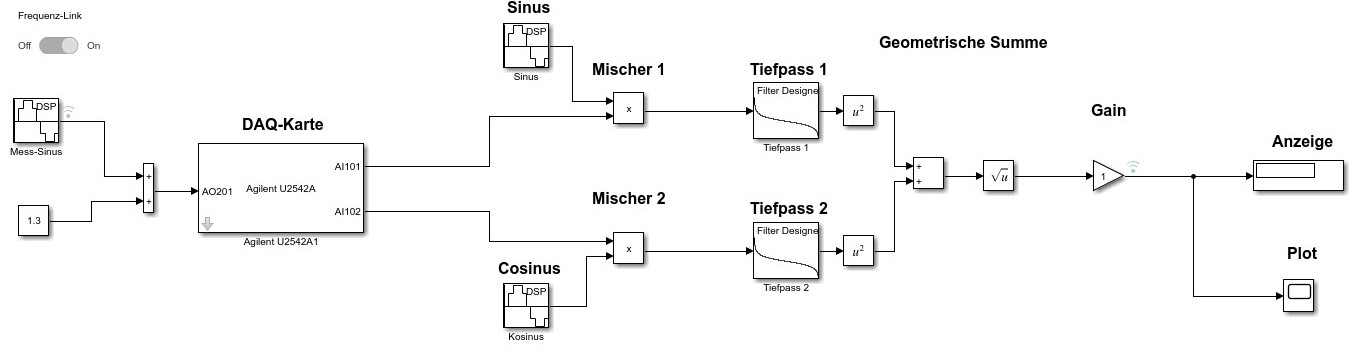
\includegraphics[width=0.8\textwidth]{schematics/6.3.6)schaltung.jpg}
    \caption{Blockschaltbild mit Konfiguration nach dem Skriptum}
    \label{fig:schematics-6-3-6-schaltung-jpg}
\end{figure}

\subsection{Messergebnisse}
Hier sind wieder die gleichen Phänomene wie bei dem phasenselektiven Synchrongleichrichter zu erwarten.
Jedoch treten bei $22\unit{Hz}$ Störungen auf, wie aus Abb. \ref{fig:images-6-3-6-22hz-jpg} ersichtlich ist.
Diese Störungen konnten nicht erklärt werden. Bis auf diese sonderbare Frequenz
alle Situationen wie in Tabelle \ref{tab:6-3-6-störfrequenz} vorhersagbar abgelaufen.

\begin{table}[h]
    \centering
    \caption{Korrespondenztabelle zwischen Störsignal und Frequenz}
    \label{tab:6-3-6-störfrequenz}
    \begin{tabular}{|c||c|c|c|}
        \hline
        Frequenz (Hz) & Störung erwartet? & Störung gemessen? & Begründung \\
        \hline
        20\pm 1 & Nein & Ja & siehe Abb. \ref{fig:images-6-3-6-22hz-jpg}; der Grund dafür ist unklar\\
        33,33 \pm 1 & Nein & Nein & Frequenzdifferenz zu hoch\\
        50 \pm 1 & Nein & Nein & Frequenzdiffernz zu hoch\\
        75 \pm 1 & Nein & Nein & Frequenzdifferenz zu hoch\\
        100 \pm 2 & Ja & Ja & $\Delta f=f - f_{Netz} = 2\unit{Hz}$; siehe Abb. \ref{fig:images-6-3-6-101hz-jpg}\\
        125 \pm 1 & Nein & Nein & Frequenzdifferenz zu hoch\\
        150 \pm 1 & Nein & Nein & Frequenzdifferenz zu hoch\\
        175 \pm 1 & Nein & Nein & Frequenzdifferenz zu hoch\\
        200 \pm 1 & Nein & Nein & Frequenzdifferenz zu hoch\\
        \hline
    \end{tabular}
\end{table}

\begin{figure}[h]
    \centering
    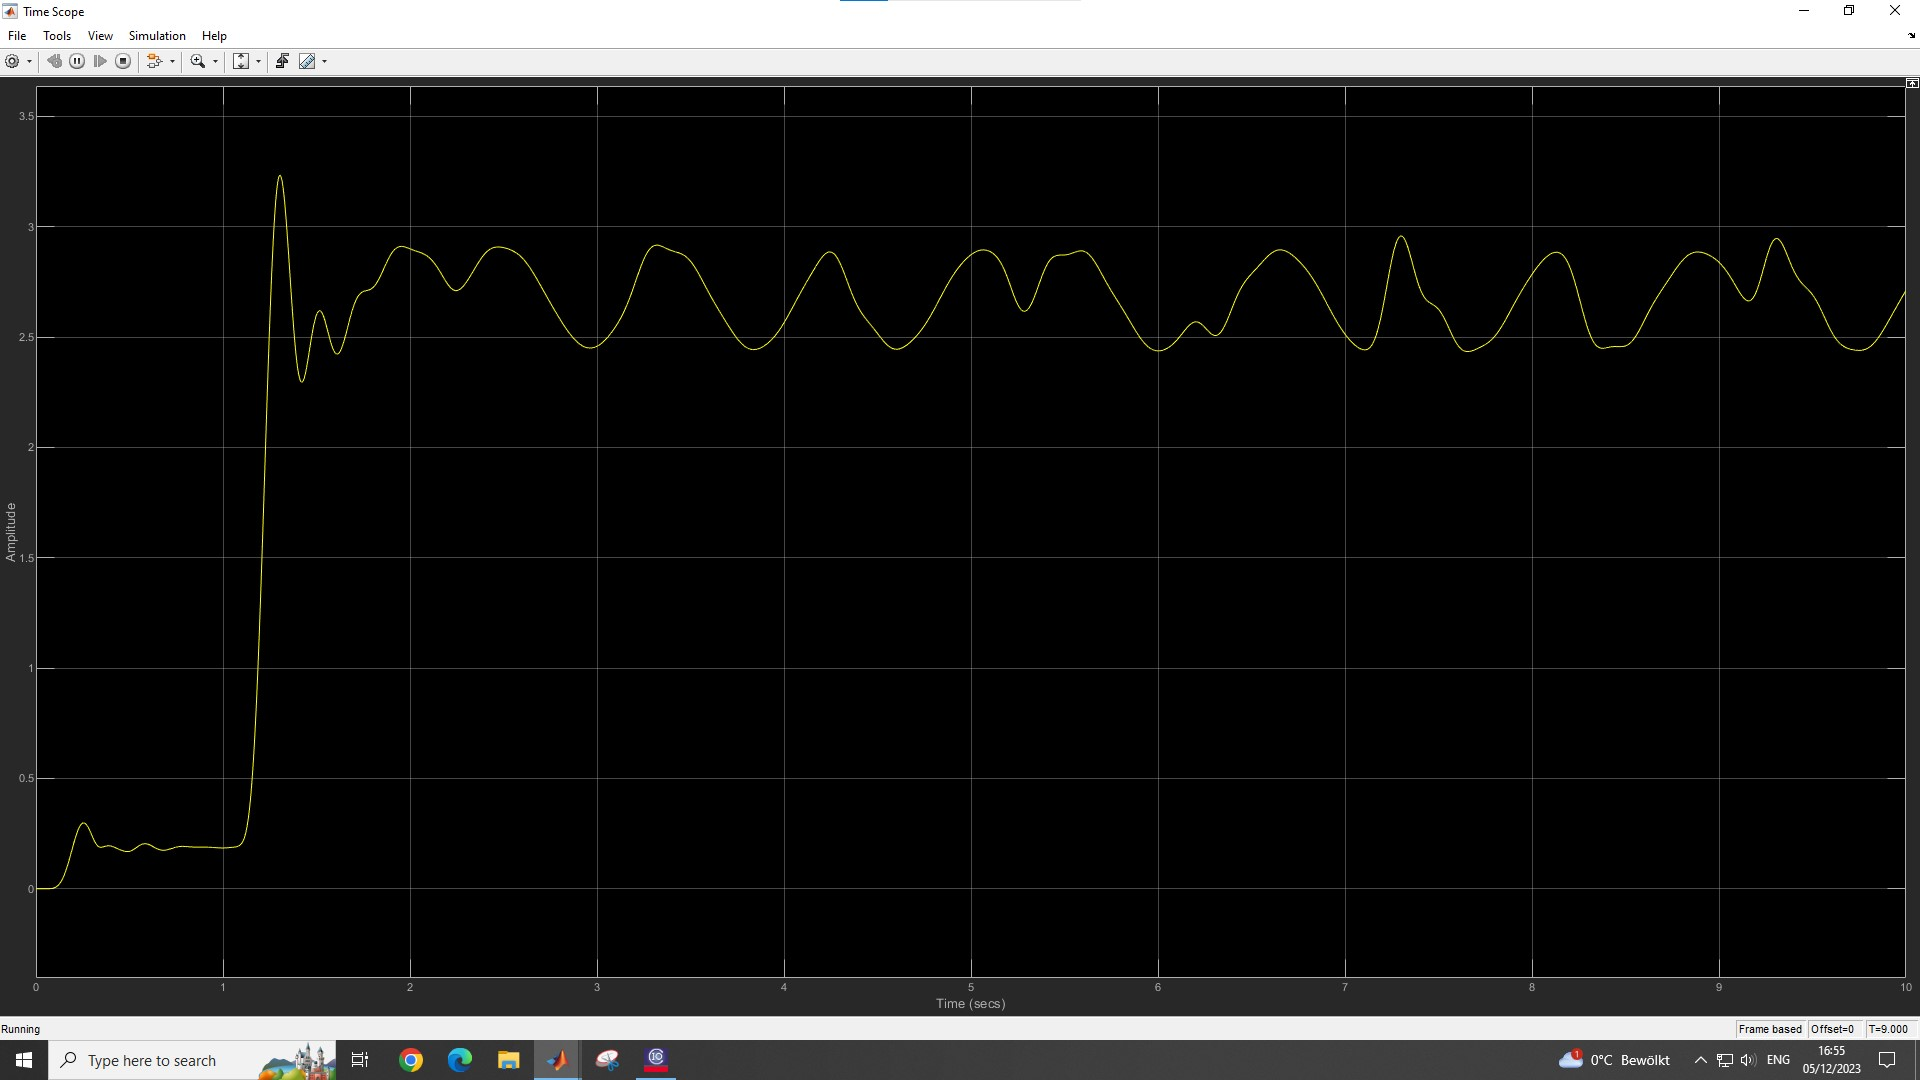
\includegraphics[width=0.8\textwidth]{images/6.3.6)101hz.jpg}
    \caption{Störungen bei einer $101\unit{Hz}$ Transiente}
    \label{fig:images-6-3-6-101hz-jpg}
\end{figure}

\begin{figure}[h]
    \centering
    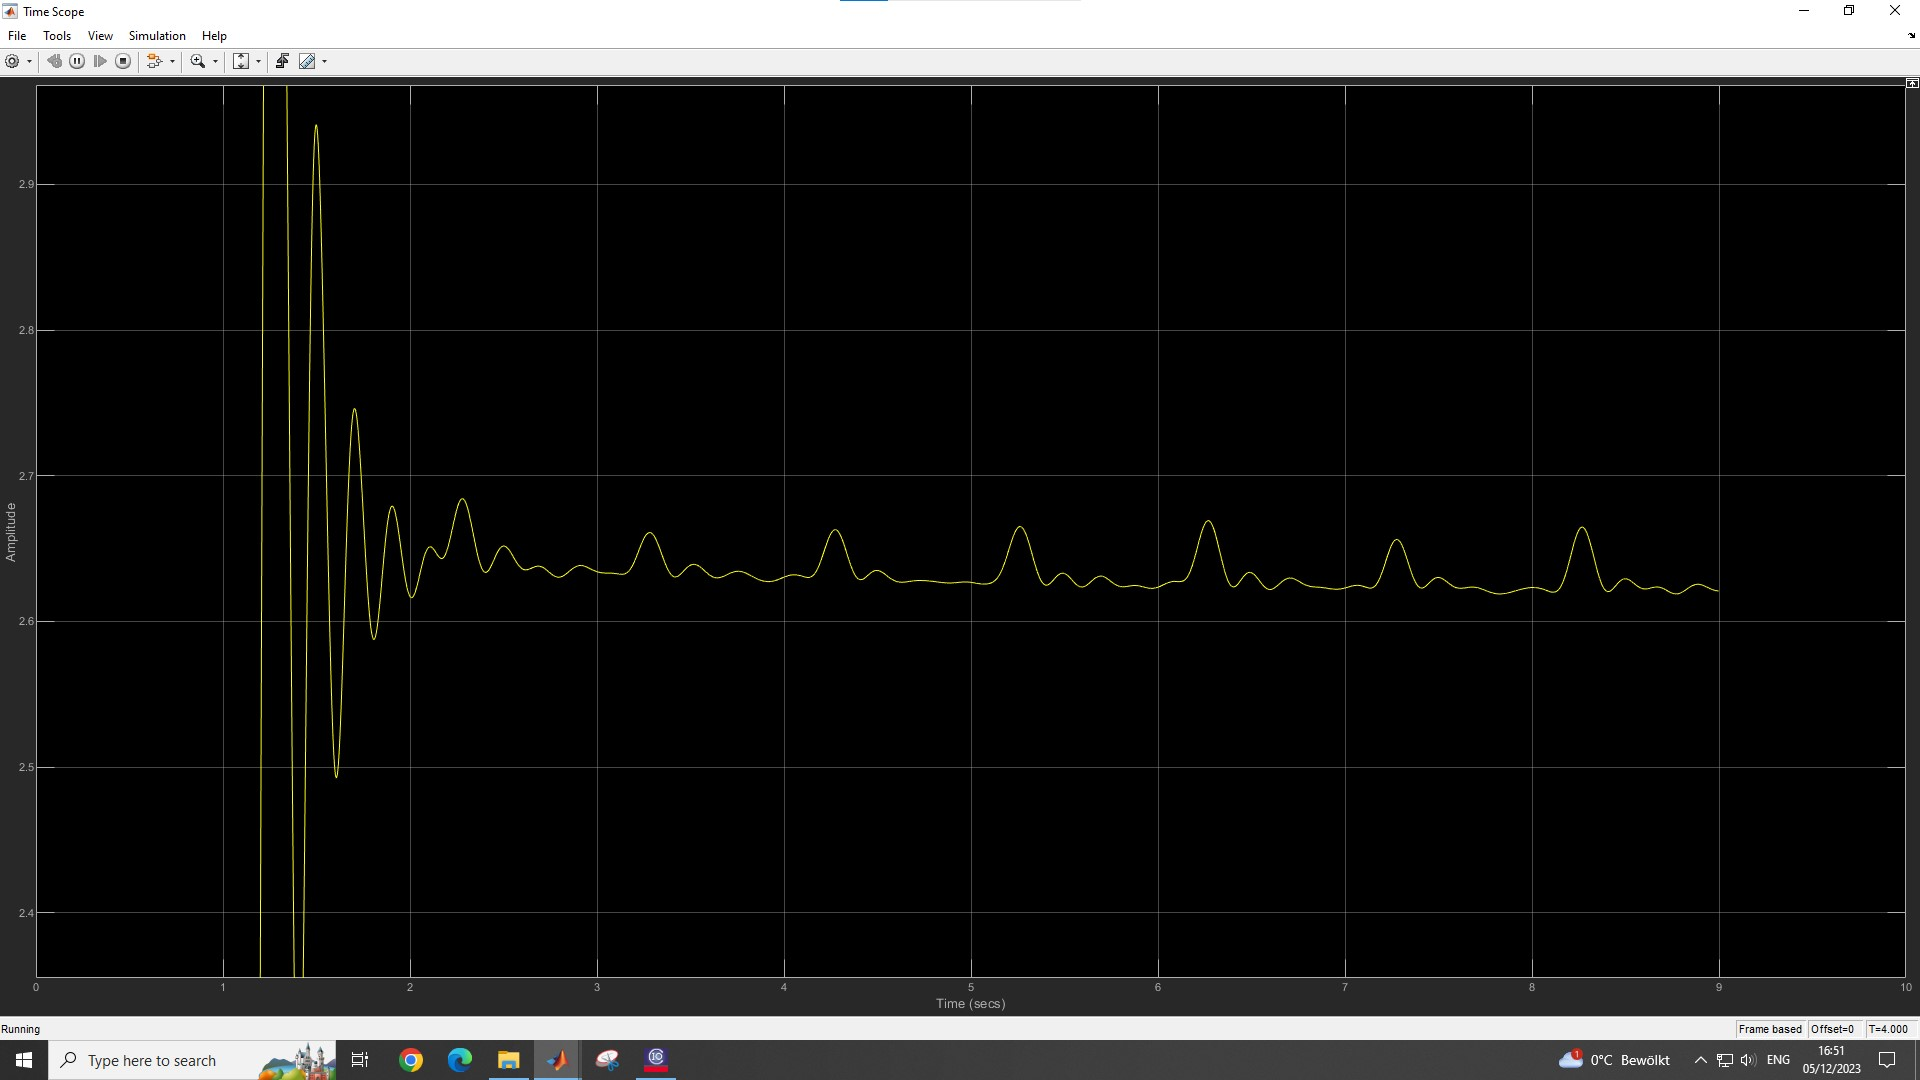
\includegraphics[width=0.8\textwidth]{images/6.3.6)22hz.jpg}
    \caption{Störungen mit $1\unit{Hz}$ Frequenz}
    \label{fig:images-6-3-6-22hz-jpg}
\end{figure}

\end{document}
